\chapter{Tracker}

We consider a tracker to be an algorithm for detection a position of an object in
an image. We present a few tested trackers and their results in this task.
Firstly, we provide a short description of a simple straightforward tracker and
then we describe more complicated trackers.

Tracker returns an object position in the image. We differentiate between two
types of tracking algorithms: \emph{detection-based algorithms} and
\emph{sequence-based algorithms}. Detection based algorithms detect an object
on each image separately. On the other hand, sequence-based algorithms obtain,
store and process information from a sequence of the past images and use them
for more accurate tracking, while requiring same or even less computation time
compared to the detection-based algorithms. For this task, we test few trackers
in both categories. Evaluation of the trackers is at the end of this chapter.

%%%%%%%%%%%%%%%%%%%%%%%%%%%%%%%%%%%%%%%%%%%%%

\section {Detection based algorithms}

We denote all trackers, which detect an object on each image separately, as
detection-based algorithms. These algorithms use only information obtained from
the current image and the information from the image used while the tracker was
initialized.

\subsection{Simple Background Tracker}

\emph{Simple Background Tracker} takes a photo of the background at the
beginning and we denote it as a \emph{pattern}. In order to detect an object in
an \emph{image}, a comparison of the \emph{image} and the \emph{pattern} is done.
We make this comparison by taking a sum of an absolute difference for each
color channel (Red, Green, Blue) in the images for each pixel.

As a result, we get a mask, where higher values mean the bigger difference between
the colors of the \emph{pattern} and the \emph{image} at given pixel. We assume it
is caused by an object in front of the camera.

One may expect to get the mask by \emph{tresholding} (see the results in
\ref{fig:simple-background-first-threshold}). There is still a lot of noise.
The noise is in the form of small dots and lines. Therefore we use
\emph{blurring} to remove the noise. Then we \emph{threshold} it again to get
binary mask (see the results in \ref{fig:simple-background-second-threshold}).
At this point, we will find a contour with the biggest area using OpenCV
library. The center point of the rectangle of this contour will be our
estimation of the position of our object in the image. The whole process is in
the figure \ref{fig:simple-background-tracker}.

In the image, it is showed that between the photo of the background and the photo
of the object the light slightly changed (at the edge of the puzzle pieces). It
is causing noise, which we reduce by thresholding and blurring the image.

\begin{figure}
  \centering
  \begin{subfigure}[b]{0.48\linewidth}
    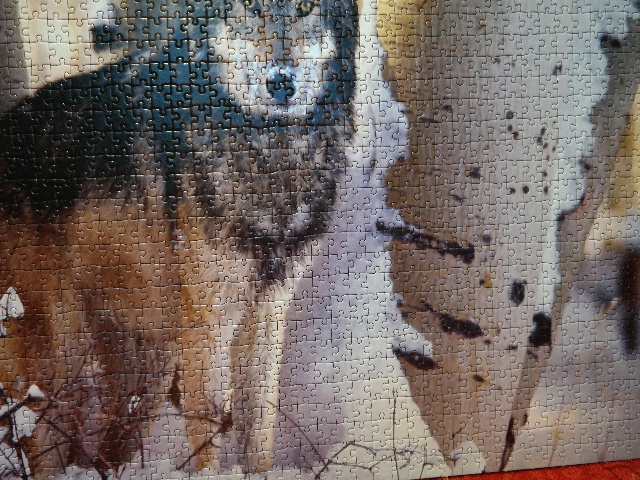
\includegraphics[width=\linewidth]{img/simple_background/background.jpg}
    \caption{Background}
  \end{subfigure}
  \begin{subfigure}[b]{0.48\linewidth}
    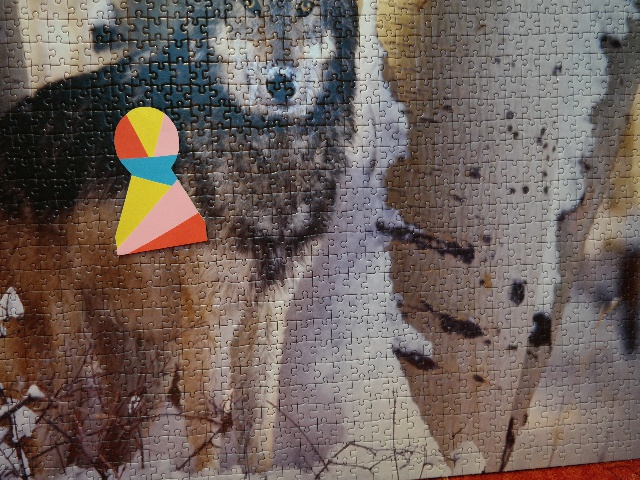
\includegraphics[width=\linewidth]{img/simple_background/object.jpg}
    \caption{Object}
  \end{subfigure}
  \begin{subfigure}[b]{0.48\linewidth}
    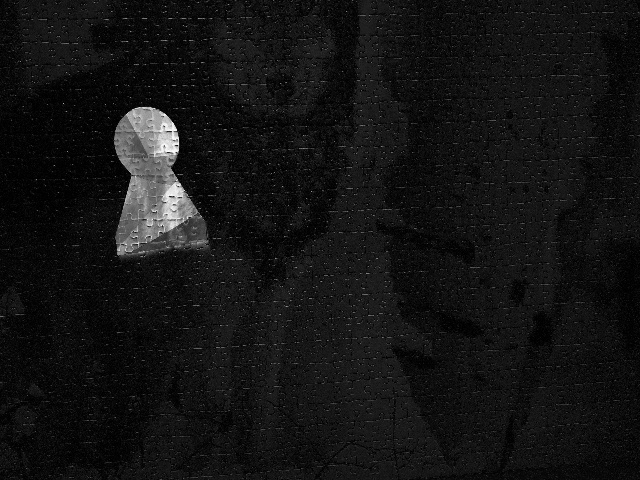
\includegraphics[width=\linewidth]{img/simple_background/rgb-diff.jpg}
    \caption{Sum of diffs in each channel (RGB)}
  \end{subfigure}
  \begin{subfigure}[b]{0.48\linewidth}
    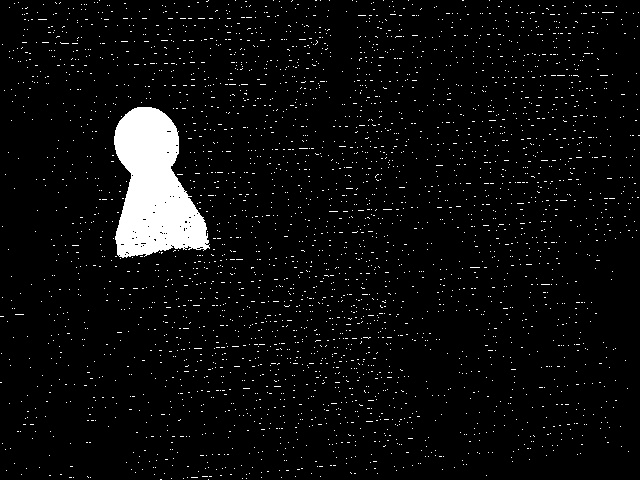
\includegraphics[width=\linewidth]{img/simple_background/first-thresh.jpg}
    \caption{Thresholded}
    \label{fig:simple-background-first-threshold}
  \end{subfigure}
  \begin{subfigure}[b]{0.48\linewidth}
    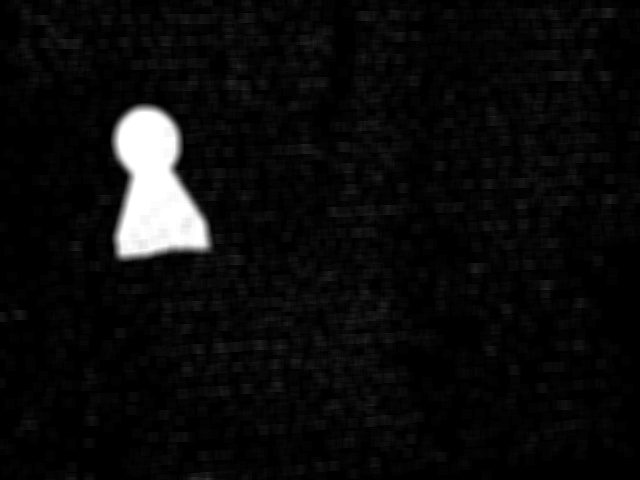
\includegraphics[width=\linewidth]{img/simple_background/blurring.jpg}
    \caption{Blurred}
  \end{subfigure}
  \begin{subfigure}[b]{0.48\linewidth}
    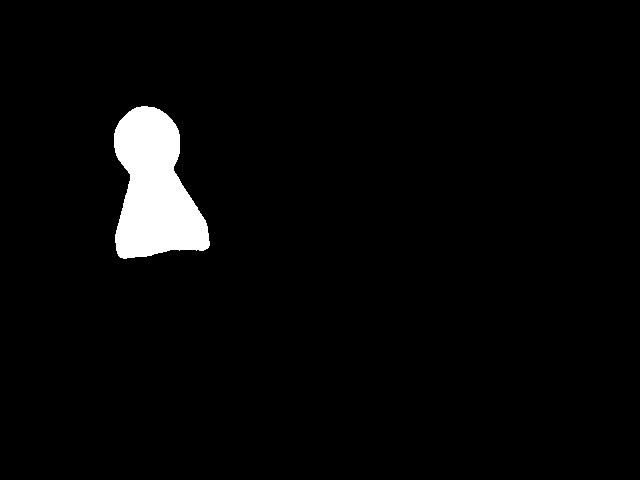
\includegraphics[width=\linewidth]{img/simple_background/second-thresh.jpg}
    \caption{Thresholded}
    \label{fig:simple-background-second-threshold}
  \end{subfigure}
  \begin{subfigure}[b]{0.48\linewidth}
    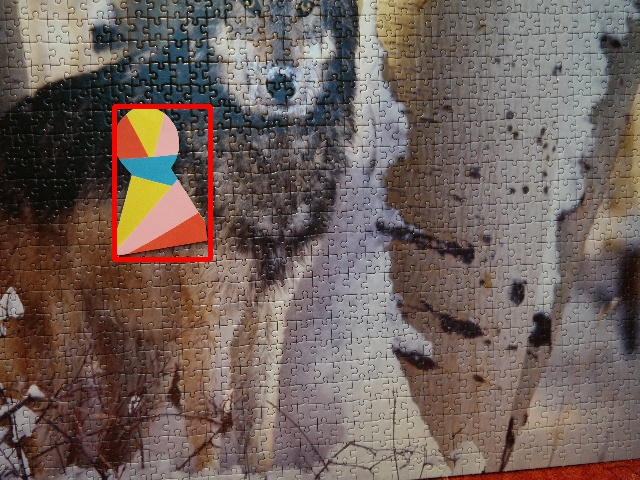
\includegraphics[width=\linewidth]{img/simple_background/result.jpg}
    \caption{Bounding box of the largest contour found.}
  \end{subfigure}
  \caption{Process of the simple background tracker}
  \label{fig:simple-background-tracker}
\end{figure}

As an advantage of this algorithm, we consider its simplicity and
straight-forward implementation. Furthermore, with a static background with
only one object moving it can reliably track an object without any information
about it.

On the contrary, it can not recover even from a little light changes or camera
movement. Also, an object moved by a human, for example, cannot be tracked
reliably, since the tracker recognizes the hand as a moving object
too.

\subsection{HSV tracker}

HSV tracker uses an idea of tracking an object by its color. Given an input
object described by a bounding box, we find the average color within the
bounding box. On a position request, we return a center of the largest area
with the color of the object.

We choose the color coding via HSV (Hue, Saturation, Value). Unlike the RGB (Red,
Green, Blue) coding it can describe a color as hue value, not triple values of
mixed colors. The approach of HSV color coding preserves one value -- hue
value,  even though the color is lighter or darker (like shadows in the image).
On the other hand in the RGB coding shadows may cause a difference in all three
parts of coded color. Therefore an object description can be simplified
to one value.

\begin{figure}[h!]\centering
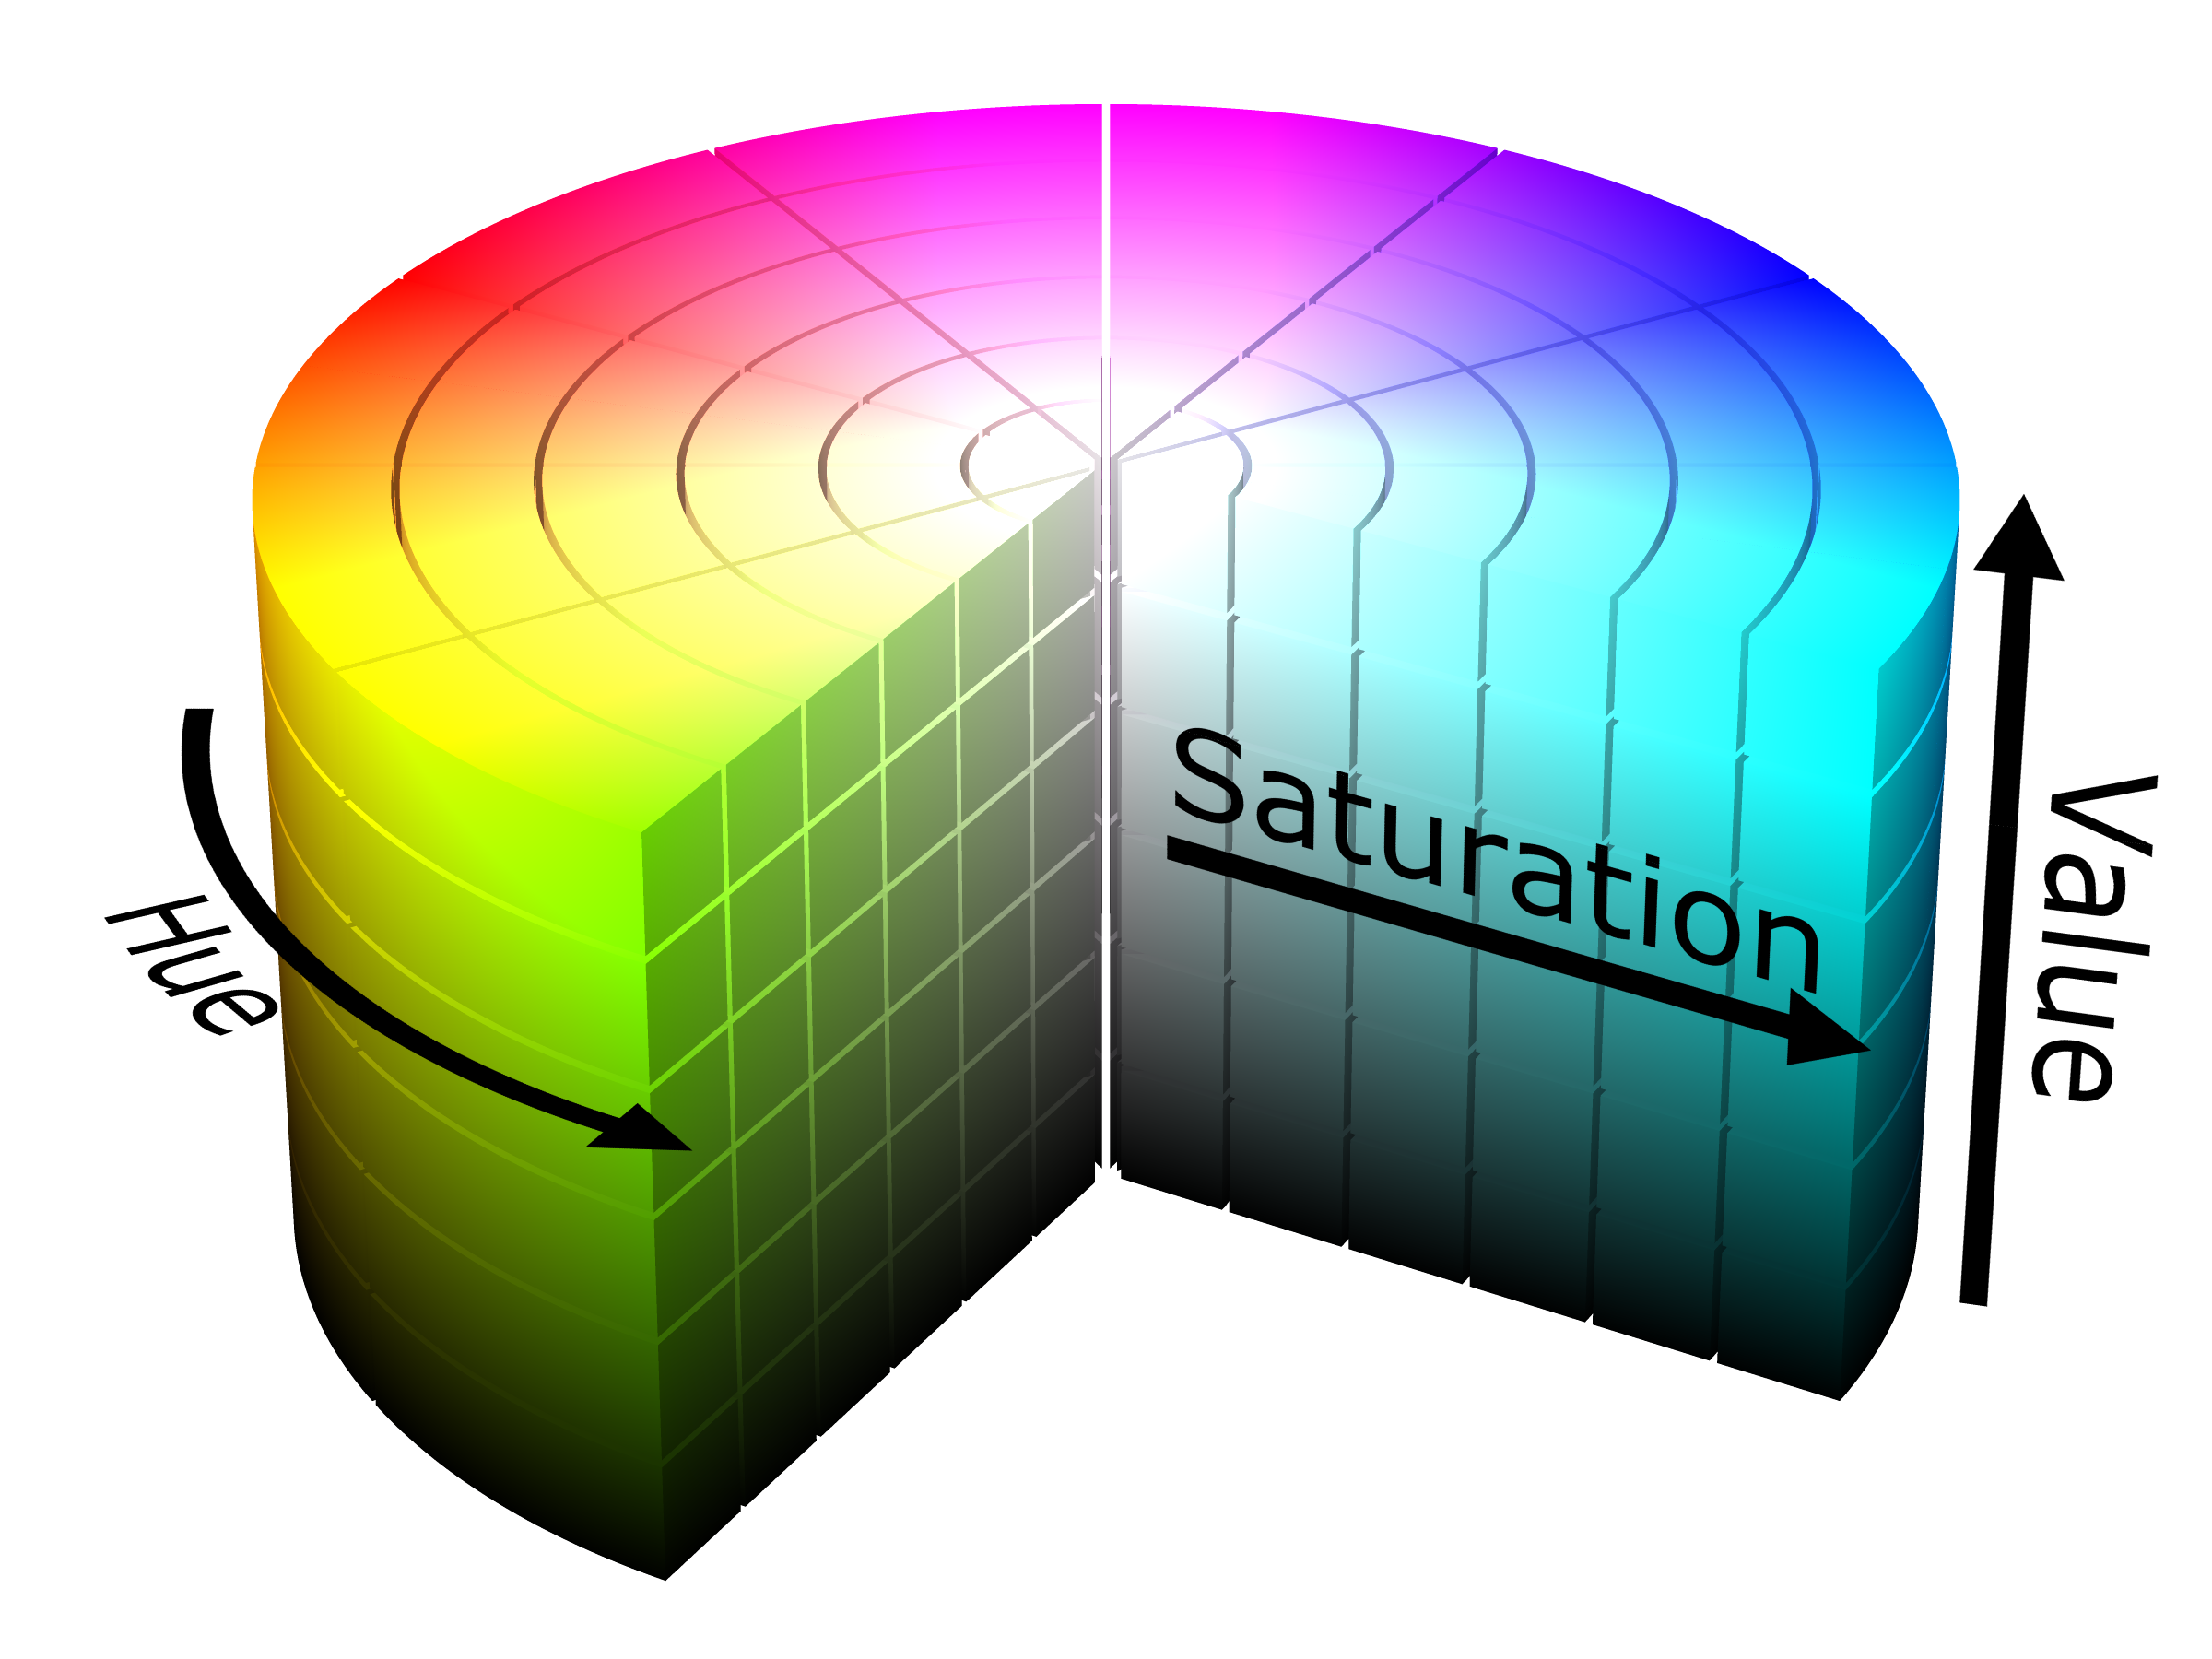
\includegraphics[width=0.65\textwidth]{img/hsv-cylinder.png}
\caption{"HSV cylinder" by SharkD is licensed under CC BY 3.0}
\end{figure}

We describe the algorithm in a few steps. Firstly, we convert the template
image (bounding box) from the RGB color space to HSV. Then we choose an average
color in the template. Since the coding of hue part is placed in the circle, it
is not enough to take a commonly used average. It would cause that image full
of warm red (the hue value of this color is circa equal to 15) and cool red
(the hue is circa 345) would average to mid cyan (hue: 180), instead of Red
(hue: 0).

To get a more reasonable average, we take the hue value of each pixel as an
unit vector (the hue value is encoded as the angle between given vector
and vector $(1, 0)$). We sum these vectors and get a vector $(x, y)$. We find a
corresponding angle for this vector using $arctang2$ function. The following
formulas describe the process of getting an average angle.

\todo[inline]{Obrazok na ten vzorceky a tak}

$$
\begin{aligned}
x &= \sum_\alpha cos \alpha \\
y &= \sum_\alpha sin \alpha \\
\alpha_{avg} &= arctang2(y, x)
\end{aligned}
$$

The use of this algorithm for one-colore object is displayed in the figure
\ref{fig:hsv-tracker}. We consider as a disadvantage that no other objects of
the same color can be placed in the view of the camera.

\begin{figure}
  \centering
  \begin{subfigure}[b]{0.48\linewidth}
    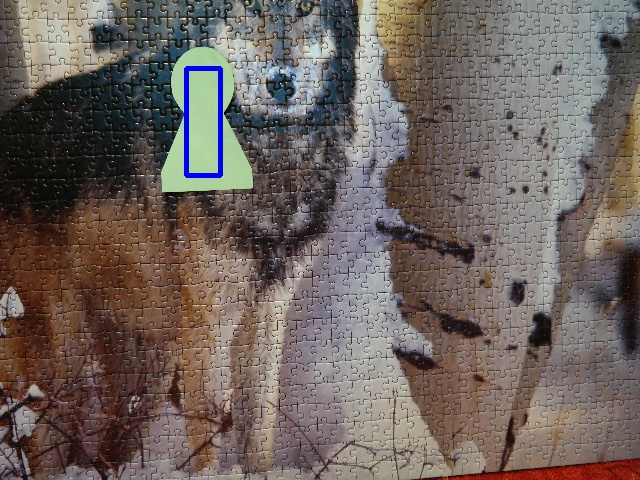
\includegraphics[width=\linewidth]{img/hsv/initial.jpg}
    \caption{Initial image with the selected object}
  \end{subfigure}
  \begin{subfigure}[b]{0.48\linewidth}
    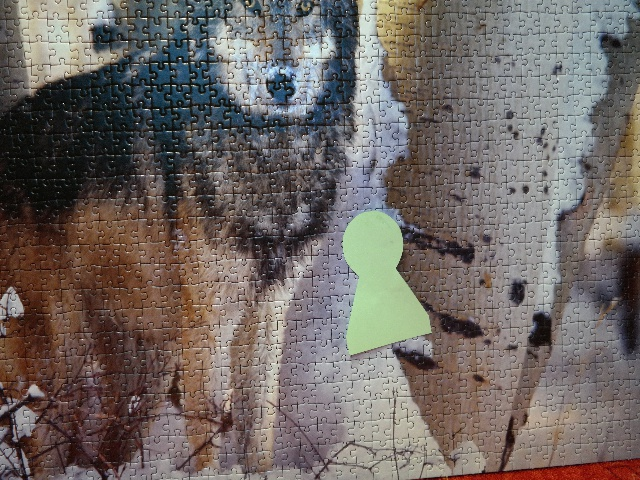
\includegraphics[width=\linewidth]{img/hsv/object.jpg}
    \caption{Image with the moved object}
  \end{subfigure}
  \begin{subfigure}[b]{0.48\linewidth}
    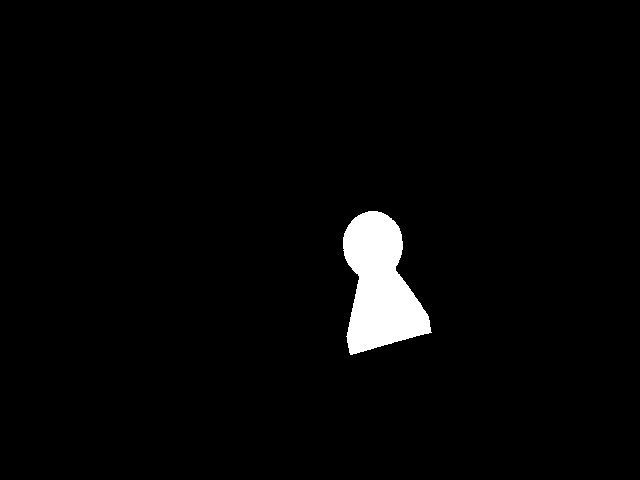
\includegraphics[width=\linewidth]{img/hsv/mask.jpg}
    \caption{Mask created by looking for similar colors}
  \end{subfigure}
  \begin{subfigure}[b]{0.48\linewidth}
    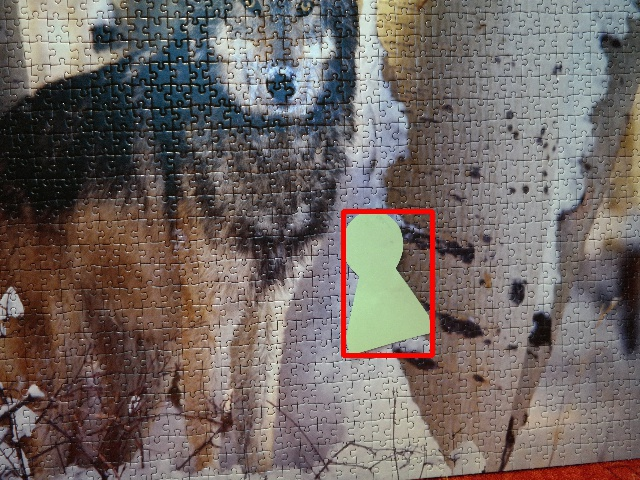
\includegraphics[width=\linewidth]{img/hsv/result.jpg}
    \caption{Bounding box of the largest contour found.}
  \end{subfigure}
  \caption{Process of the HSV tracker}
  \label{fig:hsv-tracker}
\end{figure}

\subsection {Pattern matching}

Pattern (or template) matching algorithm slides over the input image and
compares the template with the patch of the input image. By \emph{patch} we
mean an image cropped to the size of the template (displayed in the figure
\ref{fig:patternmatching-naming}).

For a comparison between the template and the patch we look for a function, which
tells us how different to each other they are. Such a function is usually called
a loss fuction. We use a function $R$ based on square distance as our loss
function. More precisely, we take the sum of square distances of all pairs of
corresponding pixels in the template and the patch. Therefore, we compute $R$
as:

$$
R(x, y) =
%\frac{
\sum_{x', y'} ||T(x', y') - I(x + x', y + y')||^2
%}{
%\sqrt{\sum_{x', y'} T(x', y')^2 \cdot \sum_{x', y'} I(x+x', y+y')^2}
%}
$$
where $x'$ and $y'$ denote points from the neighbourhood of the $x, y$. $T$
denotes our pattern and $I$ denotes the image. 

\begin{figure}[h]
	\centering
	\def\svgwidth{0.9\linewidth}
	%LaTeX with PSTricks extensions
%%Creator: inkscape 0.92.2
%%Please note this file requires PSTricks extensions
\psset{xunit=.5pt,yunit=.5pt,runit=.5pt}
\begin{pspicture}(7433.84073573,4146.76088829)
{
\newrgbcolor{curcolor}{0.99607843 0 0}
\pscustom[linewidth=37.79527559,linecolor=curcolor]
{
\newpath
\moveto(782.61759522,2305.08169451)
\lineto(1675.34199313,2305.08169451)
\lineto(1675.34199313,1094.16261079)
\lineto(782.61759522,1094.16261079)
\closepath
}
}
{
\newrgbcolor{curcolor}{0 0 0}
\pscustom[linewidth=17.57787629,linecolor=curcolor]
{
\newpath
\moveto(1671.02347843,1095.51843159)
\lineto(1918.30677921,261.95647884)
}
}
{
\newrgbcolor{curcolor}{0 0 0}
\pscustom[linestyle=none,fillstyle=solid,fillcolor=curcolor]
{
\newpath
\moveto(1734.86885202,152.21356112)
\curveto(1739.72996288,153.68925549)(1743.87492795,154.88283182)(1747.30374722,155.79429011)
\curveto(1750.73256649,156.70574839)(1753.59714968,157.42189419)(1755.89749678,157.9427275)
\curveto(1758.24124666,158.4635608)(1760.06416324,158.81078301)(1761.3662465,158.98439411)
\curveto(1762.71173255,159.20140799)(1763.70999638,159.30991493)(1764.36103802,159.30991493)
\curveto(1765.44610741,159.30991493)(1766.46607263,159.13630383)(1767.4209337,158.78908162)
\curveto(1768.37579476,158.48526219)(1769.2004475,157.9427275)(1769.8948919,157.16147754)
\curveto(1770.63273909,156.38022758)(1771.19697517,155.31685958)(1771.58760015,153.97137353)
\curveto(1771.97822513,152.66929027)(1772.17353762,151.04168618)(1772.17353762,149.08856128)
\curveto(1772.17353762,148.43751965)(1772.13013485,147.15713777)(1772.0433293,145.24741564)
\curveto(1771.99992652,143.33769352)(1771.89141958,140.69012421)(1771.71780848,137.30470771)
\curveto(1771.54419738,133.96269399)(1771.30548211,129.83943031)(1771.00166268,124.93491667)
\curveto(1770.74124603,120.07380581)(1770.39402382,114.34463943)(1769.95999607,107.74741755)
\lineto(1770.74124603,107.68231338)
\curveto(1774.12666252,116.10245184)(1777.77249567,123.54602785)(1781.67874547,130.01304142)
\curveto(1785.62839805,136.52345775)(1789.6214534,141.99220747)(1793.65791153,146.41929058)
\curveto(1797.73777244,150.84637369)(1801.79593195,154.18838741)(1805.83239008,156.44533174)
\curveto(1809.86884821,158.74567885)(1813.70999385,159.8958524)(1817.355827,159.8958524)
\curveto(1820.30721574,159.8958524)(1822.91138227,159.33161632)(1825.1683266,158.20314415)
\curveto(1827.42527093,157.11807476)(1829.37839583,155.64238039)(1831.0277013,153.77606104)
\curveto(1832.72040955,151.95314447)(1834.13099976,149.82640847)(1835.25947192,147.39585303)
\curveto(1836.38794409,145.00870038)(1837.29940237,142.49133939)(1837.99384678,139.84377008)
\curveto(1838.68829119,137.23960355)(1839.18742311,134.59203424)(1839.49124254,131.90106215)
\curveto(1839.79506197,129.21009007)(1839.94697168,126.69272908)(1839.94697168,124.3489792)
\curveto(1839.94697168,117.96877119)(1839.29593005,112.00088955)(1837.99384678,106.44533428)
\curveto(1836.69176351,100.889779)(1834.91224972,95.78995287)(1832.65530539,91.14585589)
\curveto(1830.39836106,86.54516168)(1827.72909036,82.421898)(1824.64749329,78.77606485)
\curveto(1821.56589623,75.1302317)(1818.22388251,72.04863463)(1814.62145213,69.53127365)
\curveto(1811.06242454,67.05731544)(1807.30808445,65.16929471)(1803.35843187,63.86721144)
\curveto(1799.45218207,62.5217254)(1795.52423088,61.84898237)(1791.5745783,61.84898237)
\curveto(1787.36450907,61.84898237)(1783.26294678,62.60853095)(1779.26989143,64.12762809)
\curveto(1775.27683608,65.64672524)(1771.52249599,68.16408622)(1768.00687117,71.67971104)
\curveto(1767.52944064,60.78561437)(1767.0520101,49.5442955)(1766.57457957,37.95575442)
\curveto(1766.09714904,26.32381057)(1765.83673239,14.19273479)(1765.79332961,1.5625271)
\lineto(1752.12145531,0.00002718)
\lineto(1750.75426788,0.06513134)
\curveto(1751.40530951,8.18145038)(1752.01294837,16.71009578)(1752.57718445,25.65106754)
\curveto(1753.14142053,34.54863654)(1753.66225384,43.48960831)(1754.13968437,52.47398285)
\curveto(1754.6171149,61.45835739)(1755.05114266,70.29082222)(1755.44176764,78.97137734)
\curveto(1755.83239262,87.69533523)(1756.15791343,95.87675843)(1756.41833009,103.51564693)
\curveto(1756.67874674,111.15453543)(1756.87405923,118.07727813)(1757.00426756,124.28387504)
\curveto(1757.17787866,130.53387472)(1757.26468421,135.69880502)(1757.26468421,139.77866592)
\curveto(1757.26468421,141.42797139)(1757.17787866,142.86026299)(1757.00426756,144.0755407)
\curveto(1756.83065646,145.33422119)(1756.48343425,146.37588781)(1755.96260094,147.20054054)
\curveto(1755.48517041,148.02519328)(1754.76902462,148.63283214)(1753.81416355,149.02345712)
\curveto(1752.85930249,149.45748487)(1751.600622,149.67449875)(1750.03812208,149.67449875)
\curveto(1748.43221938,149.67449875)(1746.47909448,149.50088765)(1744.17874738,149.15366544)
\curveto(1741.87840027,148.80644324)(1739.10062263,148.22050577)(1735.84541447,147.39585303)
\closepath
\moveto(1768.59280864,78.77606485)
\curveto(1772.28204456,75.65106501)(1775.9495791,73.3507179)(1779.59541225,71.87502353)
\curveto(1783.28464817,70.39932916)(1786.97388409,69.66148198)(1790.66312002,69.66148198)
\curveto(1795.52423088,69.66148198)(1799.99471677,70.6814472)(1804.07457767,72.72137766)
\curveto(1808.19784135,74.80471088)(1811.73516756,77.88630795)(1814.6865563,81.96616885)
\curveto(1817.68134781,86.04602976)(1820.00339631,91.08075172)(1821.65270178,97.07033475)
\curveto(1823.34541003,103.10332056)(1824.19176415,110.09116743)(1824.19176415,118.03387536)
\curveto(1824.19176415,120.9852641)(1823.95304888,124.02345839)(1823.47561835,127.14845823)
\curveto(1823.0415906,130.27345807)(1822.3254448,133.09463848)(1821.32718096,135.61199946)
\curveto(1820.3723199,138.17276322)(1819.09193802,140.25609645)(1817.48603532,141.86199915)
\curveto(1815.9235354,143.51130462)(1814.01381328,144.33595736)(1811.75686895,144.33595736)
\curveto(1809.10929964,144.33595736)(1806.48343171,143.64151295)(1803.87926518,142.25262413)
\curveto(1801.27509865,140.90713808)(1798.73603627,139.06252012)(1796.26207807,136.71877024)
\curveto(1793.83152263,134.41842314)(1791.48777275,131.70574966)(1789.23082842,128.58074982)
\curveto(1786.97388409,125.45574998)(1784.84714809,122.13543765)(1782.85062041,118.61981283)
\curveto(1780.85409274,115.14759078)(1779.03117616,111.54516041)(1777.38187069,107.81252171)
\curveto(1775.73256522,104.12328578)(1774.27857224,100.52085541)(1773.01989175,97.00523059)
\curveto(1771.80461403,93.48960577)(1770.80635019,90.16929344)(1770.02510023,87.0442936)
\curveto(1769.28725305,83.91929375)(1768.80982251,81.16321751)(1768.59280864,78.77606485)
\closepath
}
}
{
\newrgbcolor{curcolor}{0 0 0}
\pscustom[linestyle=none,fillstyle=solid,fillcolor=curcolor]
{
\newpath
\moveto(1907.98082144,132.29168713)
\curveto(1907.98082144,135.7205064)(1907.41658536,138.69359653)(1906.2881132,141.21095751)
\curveto(1905.15964103,143.7283185)(1903.68394666,145.78995034)(1901.86103009,147.39585303)
\curveto(1900.03811351,149.00175573)(1897.97648167,150.19533206)(1895.67613457,150.97658202)
\curveto(1893.37578746,151.75783198)(1891.07544036,152.14845696)(1888.77509325,152.14845696)
\curveto(1885.69349619,152.14845696)(1883.08932965,151.82293614)(1880.96259365,151.17189451)
\curveto(1878.83585764,150.52085287)(1877.09974662,149.63109598)(1875.75426058,148.50262381)
\curveto(1874.45217731,147.37415165)(1873.49731625,146.0286656)(1872.88967739,144.46616568)
\curveto(1872.32544131,142.94706854)(1872.04332327,141.29776306)(1872.04332327,139.51824927)
\curveto(1872.04332327,137.43491604)(1872.41224686,135.32988142)(1873.15009404,133.20314542)
\curveto(1873.931344,131.11981219)(1875.05981617,129.07988174)(1876.53551054,127.08335406)
\lineto(1876.27509389,126.36720827)
\curveto(1873.80113568,125.15193055)(1871.30547608,124.54429169)(1868.7881151,124.54429169)
\curveto(1867.31242073,124.54429169)(1865.92353191,124.76130557)(1864.62144864,125.19533333)
\curveto(1863.36276815,125.67276386)(1862.25599737,126.34550688)(1861.30113631,127.21356239)
\curveto(1860.38967803,128.0816179)(1859.65183084,129.1449859)(1859.08759476,130.4036664)
\curveto(1858.56676145,131.66234689)(1858.3063448,133.07293709)(1858.3063448,134.63543701)
\curveto(1858.3063448,137.19620077)(1858.91398366,139.60505482)(1860.12926137,141.86199915)
\curveto(1861.38794186,144.11894348)(1863.03724734,146.18057532)(1865.07717779,148.04689467)
\curveto(1867.11710824,149.91321402)(1869.48255951,151.58422088)(1872.17353159,153.05991525)
\curveto(1874.86450368,154.53560962)(1877.64228132,155.77258872)(1880.5068645,156.77085256)
\curveto(1883.37144769,157.81251917)(1886.23603088,158.59376913)(1889.10061407,159.11460244)
\curveto(1892.00860003,159.67883852)(1894.69957212,159.96095656)(1897.17353033,159.96095656)
\curveto(1901.73082176,159.96095656)(1905.61537017,159.3533177)(1908.82717557,158.13803999)
\curveto(1912.08238374,156.92276227)(1914.70825166,155.14324847)(1916.70477933,152.79949859)
\curveto(1918.74470979,150.49915149)(1920.22040416,147.69967246)(1921.13186244,144.40106152)
\curveto(1922.08672351,141.10245057)(1922.56415404,137.36981188)(1922.56415404,133.20314542)
\curveto(1922.56415404,130.33856223)(1922.43394571,127.191861)(1922.17352906,123.76304173)
\curveto(1921.95651518,120.33422246)(1921.69609853,116.73179209)(1921.3922791,112.95575061)
\curveto(1921.08845967,109.22311191)(1920.80634163,105.36026489)(1920.54592497,101.36720954)
\curveto(1920.32891109,97.37415418)(1920.22040416,93.40280022)(1920.22040416,89.45314764)
\curveto(1920.22040416,83.20314796)(1921.37057771,78.49394681)(1923.67092481,75.32554419)
\curveto(1926.01467469,72.20054435)(1929.07457037,70.63804443)(1932.85061185,70.63804443)
\curveto(1936.19262557,70.63804443)(1939.92526427,71.87502353)(1944.04852795,74.34898174)
\lineto(1945.93654868,71.54950272)
\curveto(1943.02856272,68.64151675)(1939.8601601,66.4279752)(1936.43134083,64.90887805)
\curveto(1933.00252156,63.38978091)(1929.40009119,62.63023233)(1925.62404971,62.63023233)
\curveto(1922.8028693,62.63023233)(1920.19870277,63.10766287)(1917.81155011,64.06252393)
\curveto(1915.42439745,65.01738499)(1913.36276561,66.4279752)(1911.62665459,68.29429455)
\curveto(1909.89054357,70.20401667)(1908.54505753,72.59116933)(1907.59019646,75.45575252)
\curveto(1906.6353354,78.32033571)(1906.15790487,81.64064804)(1906.15790487,85.41668951)
\curveto(1906.15790487,86.54516168)(1906.17960626,87.67363384)(1906.22300903,88.80210601)
\curveto(1906.30981458,89.93057817)(1906.4617243,91.1241545)(1906.67873818,92.38283499)
\lineto(1906.2881132,92.38283499)
\curveto(1904.42179385,88.65019629)(1902.25165507,84.96096037)(1899.77769686,81.31512722)
\curveto(1897.34714143,77.71269685)(1894.65616934,74.47919007)(1891.7047806,71.61460688)
\curveto(1888.79679464,68.79342647)(1885.6717948,66.51478075)(1882.32978108,64.77866973)
\curveto(1879.03117013,62.99915593)(1875.55894809,62.10939903)(1871.91311494,62.10939903)
\curveto(1868.91832343,62.10939903)(1866.18394856,62.63023233)(1863.70999036,63.67189895)
\curveto(1861.23603215,64.71356556)(1859.10929615,66.14585716)(1857.32978235,67.96877373)
\curveto(1855.59367132,69.7916903)(1854.22648389,71.9401277)(1853.22822006,74.4140859)
\curveto(1852.27335899,76.93144689)(1851.79592846,79.66582175)(1851.79592846,82.61721049)
\curveto(1851.79592846,86.43665474)(1852.49037287,89.90887678)(1853.87926169,93.03387663)
\curveto(1855.31155328,96.15887647)(1857.26467818,98.95835549)(1859.73863639,101.4323137)
\curveto(1862.25599737,103.90627191)(1865.25078889,106.03300791)(1868.72301094,107.81252171)
\curveto(1872.19523298,109.63543828)(1875.97127446,111.13283404)(1880.05113536,112.30470898)
\curveto(1884.13099626,113.5199867)(1888.44957243,114.4097436)(1893.00686387,114.97397968)
\curveto(1897.56415531,115.58161854)(1902.20825229,115.88543797)(1906.93915483,115.88543797)
\curveto(1907.24297426,118.61981283)(1907.48168952,121.26738214)(1907.65530063,123.8281459)
\curveto(1907.8723145,126.38890965)(1907.98082144,129.21009007)(1907.98082144,132.29168713)
\closepath
\moveto(1868.00686514,87.5651269)
\curveto(1868.00686514,85.87241866)(1868.18047624,84.24481457)(1868.52769845,82.68231465)
\curveto(1868.91832343,81.16321751)(1869.5042609,79.81773146)(1870.28551086,78.64585652)
\curveto(1871.11016359,77.47398158)(1872.13012882,76.54082191)(1873.34540653,75.8463775)
\curveto(1874.60408703,75.19533586)(1876.10148278,74.86981505)(1877.83759381,74.86981505)
\curveto(1879.79071871,74.86981505)(1881.80894777,75.32554419)(1883.892281,76.23700248)
\curveto(1885.97561423,77.14846076)(1888.01554468,78.40714126)(1890.01207236,80.01304395)
\curveto(1892.05200281,81.61894665)(1893.98342632,83.52866877)(1895.80634289,85.74221033)
\curveto(1897.67266224,87.99915466)(1899.3436691,90.45141148)(1900.81936347,93.09898079)
\curveto(1902.29505784,95.7465501)(1903.51033556,98.52432774)(1904.46519662,101.4323137)
\curveto(1905.46346046,104.38370244)(1906.11450209,107.40019534)(1906.41832152,110.48179241)
\curveto(1903.20651613,110.39498686)(1900.01641213,110.17797298)(1896.84800951,109.83075077)
\curveto(1893.67960689,109.52693134)(1890.66311399,109.02779942)(1887.7985308,108.33335502)
\curveto(1884.97735039,107.63891061)(1882.35148247,106.72745232)(1879.92092703,105.59898015)
\curveto(1877.4903716,104.47050799)(1875.38533699,103.05991778)(1873.60582319,101.36720954)
\curveto(1871.86971216,99.71790406)(1870.50252473,97.74307778)(1869.5042609,95.44273067)
\curveto(1868.50599706,93.18578634)(1868.00686514,90.55991842)(1868.00686514,87.5651269)
\closepath
}
}
{
\newrgbcolor{curcolor}{0 0 0}
\pscustom[linestyle=none,fillstyle=solid,fillcolor=curcolor]
{
\newpath
\moveto(1982.45998797,206.11980839)
\curveto(1980.63707139,197.87328103)(1979.09627286,189.34463563)(1977.83759237,180.53387218)
\curveto(1976.62231465,171.76651152)(1975.58064804,163.10765779)(1974.71259253,154.557311)
\curveto(1976.75252298,154.47050545)(1978.72734927,154.40540129)(1980.63707139,154.36199851)
\curveto(1982.59019629,154.31859574)(1984.39141148,154.27519296)(1986.04071695,154.23179019)
\curveto(1987.7334252,154.18838741)(1989.25252234,154.16668602)(1990.59800839,154.16668602)
\lineto(1994.04852905,154.16668602)
\curveto(1997.99818162,154.16668602)(2001.2316884,154.40540129)(2003.74904939,154.88283182)
\curveto(2003.96606326,154.14498464)(2004.13967437,153.47224161)(2004.26988269,152.86460276)
\curveto(2004.40009102,152.2569639)(2004.46519518,151.69272782)(2004.46519518,151.17189451)
\curveto(2004.46519518,149.26217238)(2003.66224384,148.02519328)(2002.05634114,147.4609572)
\curveto(2000.49384122,146.89672111)(1998.2151955,146.61460307)(1995.22040399,146.61460307)
\curveto(1992.3558208,146.61460307)(1989.14401541,146.78821418)(1985.58498781,147.13543638)
\curveto(1982.06936299,147.48265858)(1978.20651596,147.8081794)(1973.99644673,148.11199883)
\curveto(1973.5190162,143.46790184)(1973.10668983,138.9323118)(1972.75946763,134.50522869)
\curveto(1972.4556482,130.12154835)(1972.19523154,125.97658329)(1971.97821767,122.07033349)
\curveto(1971.80460656,118.16408368)(1971.67439824,114.53995192)(1971.58759268,111.1979382)
\curveto(1971.50078713,107.85592448)(1971.45738436,104.94793852)(1971.45738436,102.47398031)
\curveto(1971.45738436,97.82988333)(1971.69609962,93.68491826)(1972.17353016,90.03908511)
\curveto(1972.65096069,86.39325196)(1973.49731481,83.28995351)(1974.71259253,80.72918975)
\curveto(1975.92787024,78.21182877)(1977.5988771,76.28040525)(1979.72561311,74.93491921)
\curveto(1981.85234911,73.58943317)(1984.54332119,72.91669015)(1987.79852936,72.91669015)
\curveto(1990.14227924,72.91669015)(1992.74644578,73.32901651)(1995.61102897,74.15366925)
\curveto(1998.51901493,74.97832199)(2001.81762587,76.30210664)(2005.5068618,78.12502322)
\curveto(2006.67873674,76.95314827)(2007.35147976,75.52085668)(2007.52509086,73.82814843)
\curveto(2004.83411878,72.04863463)(2002.1214453,70.42103055)(1999.38707044,68.94533618)
\curveto(1996.65269558,67.51304459)(1993.96172349,66.27606548)(1991.31415418,65.23439887)
\curveto(1988.66658487,64.19273226)(1986.10582111,63.38978091)(1983.63186291,62.82554482)
\curveto(1981.1579047,62.26130874)(1978.81415482,61.9791907)(1976.60061326,61.9791907)
\curveto(1973.6926273,61.9791907)(1971.0233566,62.5217254)(1968.59280117,63.60679479)
\curveto(1966.20564851,64.6484614)(1964.12231529,66.51478075)(1962.34280149,69.20575283)
\curveto(1960.60669046,71.9401277)(1959.23950303,75.60766223)(1958.2412392,80.20835644)
\curveto(1957.28637813,84.80905065)(1956.8089476,90.62502258)(1956.8089476,97.65627222)
\curveto(1956.8089476,101.6059248)(1956.87405176,105.66408432)(1957.00426009,109.83075077)
\curveto(1957.13446842,114.04082)(1957.30807952,118.29429201)(1957.5250934,122.59116679)
\curveto(1957.74210728,126.88804157)(1958.02422532,131.18491636)(1958.37144752,135.48179114)
\curveto(1958.71866973,139.77866592)(1959.10929471,144.01043654)(1959.54332246,148.17710299)
\curveto(1956.11450319,148.13370022)(1952.92439919,147.9817905)(1949.97301045,147.72137385)
\curveto(1947.06502448,147.50435997)(1944.56936489,147.13543638)(1942.48603166,146.61460307)
\curveto(1942.35582333,146.87501973)(1942.29071917,147.17883916)(1942.29071917,147.52606136)
\curveto(1942.29071917,148.43751965)(1942.72474693,149.28387377)(1943.59280244,150.06512373)
\curveto(1944.50426073,150.88977647)(1945.74123983,151.62762365)(1947.30373975,152.27866529)
\curveto(1948.90964245,152.92970692)(1950.81936457,153.47224161)(1953.03290613,153.90626937)
\curveto(1955.24644768,154.34029713)(1957.67700311,154.64411655)(1960.32457242,154.81772766)
\curveto(1961.32283626,163.88890775)(1962.38620426,172.46095593)(1963.51467643,180.53387218)
\curveto(1964.64314859,188.60678844)(1965.77162076,195.81164919)(1966.90009292,202.14845442)
\curveto(1967.1171068,203.27692659)(1967.50773178,204.21008626)(1968.07196786,204.94793345)
\curveto(1968.67960672,205.68578063)(1969.37405113,206.2717181)(1970.15530109,206.70574586)
\curveto(1970.93655105,207.13977361)(1971.78290518,207.44359304)(1972.69436346,207.61720414)
\curveto(1973.60582175,207.79081525)(1974.49557865,207.8776208)(1975.36363416,207.8776208)
\curveto(1976.79592575,207.8776208)(1978.07630763,207.72571108)(1979.2047798,207.42189165)
\curveto(1980.37665474,207.11807222)(1981.46172413,206.68404447)(1982.45998797,206.11980839)
\closepath
}
}
{
\newrgbcolor{curcolor}{0 0 0}
\pscustom[linestyle=none,fillstyle=solid,fillcolor=curcolor]
{
\newpath
\moveto(2066.50947038,132.22658297)
\curveto(2067.72474809,134.61373563)(2068.33238695,137.04429106)(2068.33238695,139.51824927)
\curveto(2068.33238695,141.21095751)(2068.02856752,142.79515882)(2067.42092867,144.27085319)
\curveto(2066.85669258,145.78995034)(2065.98863707,147.11373499)(2064.81676213,148.24220716)
\curveto(2063.64488719,149.4140821)(2062.16919282,150.32554038)(2060.38967902,150.97658202)
\curveto(2058.653568,151.67102643)(2056.61363755,152.01824863)(2054.26988767,152.01824863)
\curveto(2050.88447117,152.01824863)(2047.84627688,151.41060977)(2045.1553048,150.19533206)
\curveto(2042.46433271,149.02345712)(2040.07718005,147.39585303)(2037.99384683,145.31251981)
\curveto(2035.95391637,143.22918658)(2034.19610396,140.82033253)(2032.72040959,138.08595767)
\curveto(2031.288118,135.35158281)(2030.09454167,132.42189546)(2029.13968061,129.29689562)
\curveto(2028.22822232,126.17189578)(2027.5554793,122.96009038)(2027.12145154,119.66147944)
\curveto(2026.68742379,116.40627127)(2026.47040991,113.21616727)(2026.47040991,110.09116743)
\curveto(2026.47040991,104.49220938)(2027.18655571,99.39238325)(2028.6188473,94.79168904)
\curveto(2030.09454167,90.2343976)(2032.06936796,86.3281478)(2034.54332617,83.07293963)
\curveto(2037.01728437,79.86113424)(2039.90356895,77.36547464)(2043.20217989,75.58596084)
\curveto(2046.50079084,73.80644705)(2050.01641566,72.91669015)(2053.74905436,72.91669015)
\curveto(2057.69870694,72.91669015)(2061.69176229,73.93665537)(2065.72822042,75.97658582)
\curveto(2069.80808132,78.05991905)(2073.7577339,81.40193277)(2077.57717815,86.00262698)
\curveto(2077.8375948,85.87241866)(2078.16311562,85.67710617)(2078.5537406,85.41668951)
\curveto(2078.98776836,85.19967563)(2079.37839334,84.93925898)(2079.72561554,84.63543955)
\curveto(2080.07283775,84.33162012)(2080.37665717,84.02780069)(2080.63707383,83.72398126)
\curveto(2080.89749048,83.42016184)(2081.02769881,83.13804379)(2081.02769881,82.87762714)
\curveto(2081.02769881,82.70401604)(2081.00599742,82.5955091)(2080.96259464,82.55210632)
\lineto(2080.83238632,82.29168967)
\curveto(2076.62231709,75.47745391)(2071.56589373,70.37762777)(2065.66311625,66.99221128)
\curveto(2059.76033878,63.60679479)(2053.29332522,61.91408654)(2046.26207557,61.91408654)
\curveto(2042.44263132,61.91408654)(2038.9270065,62.45662123)(2035.71520111,63.54169062)
\curveto(2032.50339572,64.58335724)(2029.59540975,66.03735022)(2026.99124322,67.90366957)
\curveto(2024.38707668,69.81339169)(2022.08672958,72.04863463)(2020.0902019,74.60939839)
\curveto(2018.137077,77.21356493)(2016.48777153,80.01304395)(2015.14228548,83.00783547)
\curveto(2013.84020222,86.04602976)(2012.84193838,89.21443237)(2012.14749397,92.51304332)
\curveto(2011.49645234,95.85505704)(2011.17093152,99.21877214)(2011.17093152,102.60418864)
\curveto(2011.17093152,107.16148007)(2011.67006344,111.71877151)(2012.66832728,116.27606295)
\curveto(2013.66659112,120.87675716)(2015.1205841,125.28213888)(2017.03030622,129.49220811)
\curveto(2018.98343112,133.74568011)(2021.327181,137.69533269)(2024.06155587,141.34116584)
\curveto(2026.8393335,145.03040176)(2029.96433334,148.22050577)(2033.43655539,150.91147785)
\curveto(2036.95218021,153.64585272)(2040.81502724,155.77258872)(2045.02509647,157.29168586)
\curveto(2049.2351657,158.85418579)(2053.72735297,159.63543575)(2058.50165828,159.63543575)
\curveto(2062.06068588,159.63543575)(2065.38099821,159.20140799)(2068.46259528,158.33335248)
\curveto(2071.54419234,157.46529697)(2074.19176166,156.22831786)(2076.40530321,154.62241517)
\curveto(2078.66224754,153.05991525)(2080.42005995,151.15019312)(2081.67874044,148.89324879)
\curveto(2082.98082371,146.67970724)(2083.63186534,144.20574903)(2083.63186534,141.47137417)
\curveto(2083.63186534,139.69186037)(2083.3497473,138.10765906)(2082.78551122,136.71877024)
\curveto(2082.26467791,135.3732842)(2081.50512934,134.20140926)(2080.5068655,133.20314542)
\curveto(2079.55200444,132.24828436)(2078.40183089,131.51043717)(2077.05634484,130.98960387)
\curveto(2075.75426158,130.51217333)(2074.32196998,130.27345807)(2072.75947006,130.27345807)
\curveto(2071.804609,130.27345807)(2070.80634516,130.36026362)(2069.76467855,130.53387472)
\curveto(2068.76641471,130.7508886)(2067.76815087,131.07640942)(2066.76988703,131.51043717)
\closepath
}
}
{
\newrgbcolor{curcolor}{0 0 0}
\pscustom[linestyle=none,fillstyle=solid,fillcolor=curcolor]
{
\newpath
\moveto(2113.97038824,99.93491794)
\curveto(2117.31240196,110.91582016)(2120.84972817,120.22571552)(2124.58236687,127.86460402)
\curveto(2128.35840835,135.50349253)(2132.1778526,141.68838805)(2136.04069962,146.41929058)
\curveto(2139.94694943,151.1935959)(2143.83149784,154.64411655)(2147.69434487,156.77085256)
\curveto(2151.55719189,158.89758856)(2155.24642782,159.96095656)(2158.76205264,159.96095656)
\curveto(2161.19260807,159.96095656)(2163.53635795,159.48352603)(2165.79330228,158.52866497)
\curveto(2168.05024661,157.61720668)(2170.04677429,156.18491509)(2171.78288531,154.23179019)
\curveto(2173.56239911,152.27866529)(2174.97298932,149.7613043)(2176.01465593,146.67970724)
\curveto(2177.05632254,143.59811017)(2177.57715585,139.90887425)(2177.57715585,135.61199946)
\curveto(2177.57715585,134.3099162)(2177.4903503,132.5304024)(2177.3167392,130.27345807)
\curveto(2177.18653087,128.05991651)(2177.01291977,125.56425692)(2176.79590589,122.78647928)
\curveto(2176.57889201,120.05210442)(2176.31847536,117.16581985)(2176.01465593,114.12762555)
\curveto(2175.75423928,111.08943126)(2175.51552401,108.09463975)(2175.29851013,105.14325101)
\curveto(2175.08149625,102.19186227)(2174.88618376,99.39238325)(2174.71257266,96.74481394)
\curveto(2174.58236433,94.09724463)(2174.51726017,91.81859891)(2174.51726017,89.90887678)
\curveto(2174.51726017,86.52346029)(2174.6474685,83.76738404)(2174.90788515,81.64064804)
\curveto(2175.21170458,79.51391203)(2175.68913511,77.82120379)(2176.34017675,76.56252329)
\curveto(2176.99121838,75.34724558)(2177.85927389,74.50089145)(2178.94434328,74.02346092)
\curveto(2180.02941267,73.58943317)(2181.35319732,73.37241929)(2182.91569725,73.37241929)
\curveto(2185.17264158,73.37241929)(2187.51639146,73.67623872)(2189.94694689,74.28387758)
\curveto(2192.37750232,74.93491921)(2194.82975914,75.82467611)(2197.30371735,76.95314827)
\lineto(2198.54069645,73.56773178)
\curveto(2196.97819653,72.30905129)(2195.00337024,71.02866941)(2192.61621759,69.72658614)
\curveto(2190.22906493,68.42450287)(2187.71170395,67.23092655)(2185.06413464,66.14585716)
\curveto(2182.4599681,65.06078777)(2179.85580157,64.19273226)(2177.25163503,63.54169062)
\curveto(2174.6474685,62.84724621)(2172.34712139,62.50002401)(2170.35059372,62.50002401)
\curveto(2168.00684384,62.50002401)(2166.16222587,63.12936425)(2164.81673983,64.38804475)
\curveto(2163.47125379,65.64672524)(2162.45128856,67.36113487)(2161.75684415,69.53127365)
\curveto(2161.10580252,71.70141243)(2160.67177476,74.2404748)(2160.45476089,77.14846076)
\curveto(2160.28114978,80.05644673)(2160.19434423,83.18144657)(2160.19434423,86.52346029)
\curveto(2160.19434423,90.55991842)(2160.32455256,94.72658487)(2160.58496921,99.02345965)
\curveto(2160.88878864,103.32033444)(2161.19260807,107.44359812)(2161.4964275,111.39325069)
\curveto(2161.8436497,115.34290327)(2162.14746913,118.94533364)(2162.40788579,122.20054181)
\curveto(2162.71170522,125.49915276)(2162.86361493,128.14672207)(2162.86361493,130.14324974)
\curveto(2162.86361493,134.96095783)(2161.93045525,138.5633882)(2160.06413591,140.95054086)
\curveto(2158.19781656,143.38109629)(2155.68045557,144.59637401)(2152.51205295,144.59637401)
\curveto(2150.03809475,144.59637401)(2147.39052544,143.53300601)(2144.56934502,141.40627)
\curveto(2141.79156739,139.279534)(2139.01378975,136.34984665)(2136.23601211,132.61720795)
\curveto(2133.50163725,128.92797203)(2130.85406794,124.54429169)(2128.29330418,119.46616695)
\curveto(2125.73254042,114.43144498)(2123.43219332,108.96269526)(2121.39226287,103.05991778)
\curveto(2119.35233242,97.20054308)(2117.65962417,91.05905034)(2116.31413813,84.63543955)
\curveto(2114.96865208,78.21182877)(2114.12229796,71.78821798)(2113.77507575,65.3646072)
\lineto(2099.90788896,63.67189895)
\lineto(2098.86622234,63.73700311)
\curveto(2099.126639,68.85853063)(2099.40875704,74.50089145)(2099.71257647,80.66408559)
\curveto(2100.05979867,86.87068249)(2100.40702088,93.44620299)(2100.75424308,100.39064709)
\curveto(2101.14486806,107.33509118)(2101.53549304,114.56165331)(2101.92611802,122.07033349)
\curveto(2102.36014578,129.62241644)(2102.77247215,137.30470771)(2103.16309713,145.11720732)
\curveto(2103.59712488,152.92970692)(2104.03115264,160.80731069)(2104.46518039,168.75001862)
\curveto(2104.89920815,176.69272655)(2105.31153452,184.52692754)(2105.7021595,192.25262159)
\curveto(2106.13618725,200.02171842)(2106.54851362,207.61720414)(2106.9391386,215.03907877)
\curveto(2107.32976358,222.46095339)(2107.69868717,229.5573072)(2108.04590938,236.32814019)
\curveto(2108.08931215,237.3698068)(2108.39313158,238.2595637)(2108.95736767,238.99741088)
\curveto(2109.52160375,239.77866085)(2110.23774954,240.3862997)(2111.10580506,240.82032746)
\curveto(2112.01726334,241.29775799)(2113.03722857,241.64498019)(2114.16570073,241.86199407)
\curveto(2115.2941729,242.07900795)(2116.46604784,242.18751489)(2117.68132556,242.18751489)
\curveto(2120.28549209,242.18751489)(2123.01986695,241.49307048)(2125.88445014,240.10418166)
\curveto(2124.8861863,231.25001544)(2123.9964294,223.11199502)(2123.21517944,215.6901204)
\curveto(2122.43392948,208.31164855)(2121.71778368,201.45401001)(2121.06674205,195.11720478)
\curveto(2120.45910319,188.82380232)(2119.89486711,182.94272623)(2119.3740338,177.47397651)
\curveto(2118.89660327,172.00522678)(2118.44087413,166.75349094)(2118.00684637,161.71876897)
\curveto(2117.61622139,156.72744978)(2117.2472978,151.84463753)(2116.9000756,147.07033222)
\curveto(2116.55285339,142.2960269)(2116.20563119,137.43491604)(2115.85840898,132.48699962)
\curveto(2115.51118678,127.58248598)(2115.14226318,122.46095847)(2114.7516382,117.12241707)
\curveto(2114.404416,111.82727845)(2114.01379102,106.11981346)(2113.57976326,100.00002211)
\closepath
}
}
{
\newrgbcolor{curcolor}{0 0 0}
\pscustom[linestyle=none,fillstyle=solid,fillcolor=curcolor]
{
\newpath
\moveto(6682.68938467,1343.49043349)
\curveto(6680.86646809,1335.24390613)(6679.32566956,1326.71526073)(6678.06698907,1317.90449729)
\curveto(6676.85171135,1309.13713662)(6675.81004474,1300.47828289)(6674.94198923,1291.92793611)
\curveto(6676.98191968,1291.84113055)(6678.95674597,1291.77602639)(6680.86646809,1291.73262362)
\curveto(6682.819593,1291.68922084)(6684.62080818,1291.64581806)(6686.27011365,1291.60241529)
\curveto(6687.9628219,1291.55901251)(6689.48191905,1291.53731113)(6690.82740509,1291.53731113)
\lineto(6694.27792575,1291.53731113)
\curveto(6698.22757832,1291.53731113)(6701.46108511,1291.77602639)(6703.97844609,1292.25345692)
\curveto(6704.19545997,1291.51560974)(6704.36907107,1290.84286672)(6704.4992794,1290.23522786)
\curveto(6704.62948772,1289.627589)(6704.69459189,1289.06335292)(6704.69459189,1288.54251961)
\curveto(6704.69459189,1286.63279749)(6703.89164054,1285.39581838)(6702.28573784,1284.8315823)
\curveto(6700.72323792,1284.26734622)(6698.4445922,1283.98522818)(6695.44980069,1283.98522818)
\curveto(6692.5852175,1283.98522818)(6689.37341211,1284.15883928)(6685.81438451,1284.50606148)
\curveto(6682.29875969,1284.85328369)(6678.43591266,1285.1788045)(6674.22584343,1285.48262393)
\curveto(6673.7484129,1280.83852695)(6673.33608653,1276.3029369)(6672.98886433,1271.87585379)
\curveto(6672.6850449,1267.49217346)(6672.42462825,1263.34720839)(6672.20761437,1259.44095859)
\curveto(6672.03400327,1255.53470879)(6671.90379494,1251.91057703)(6671.81698939,1248.56856331)
\curveto(6671.73018384,1245.22654959)(6671.68678106,1242.31856362)(6671.68678106,1239.84460542)
\curveto(6671.68678106,1235.20050843)(6671.92549633,1231.05554336)(6672.40292686,1227.40971021)
\curveto(6672.88035739,1223.76387706)(6673.72671151,1220.66057861)(6674.94198923,1218.09981485)
\curveto(6676.15726694,1215.58245387)(6677.8282738,1213.65103036)(6679.95500981,1212.30554431)
\curveto(6682.08174581,1210.96005827)(6684.7727179,1210.28731525)(6688.02792606,1210.28731525)
\curveto(6690.37167595,1210.28731525)(6692.97584248,1210.69964162)(6695.84042567,1211.52429435)
\curveto(6698.74841163,1212.34894709)(6702.04702258,1213.67273174)(6705.7362585,1215.49564832)
\curveto(6706.90813344,1214.32377338)(6707.58087646,1212.89148178)(6707.75448756,1211.19877354)
\curveto(6705.06351548,1209.41925974)(6702.350842,1207.79165565)(6699.61646714,1206.31596128)
\curveto(6696.88209228,1204.88366969)(6694.1911202,1203.64669059)(6691.54355089,1202.60502397)
\curveto(6688.89598158,1201.56335736)(6686.33521782,1200.76040601)(6683.86125961,1200.19616993)
\curveto(6681.3873014,1199.63193384)(6679.04355152,1199.3498158)(6676.83000997,1199.3498158)
\curveto(6673.922024,1199.3498158)(6671.2527533,1199.8923505)(6668.82219787,1200.97741989)
\curveto(6666.43504522,1202.0190865)(6664.35171199,1203.88540585)(6662.57219819,1206.57637794)
\curveto(6660.83608717,1209.3107528)(6659.46889974,1212.97828733)(6658.4706359,1217.57898155)
\curveto(6657.51577484,1222.17967576)(6657.0383443,1227.99564768)(6657.0383443,1235.02689733)
\curveto(6657.0383443,1238.9765499)(6657.10344847,1243.03470942)(6657.23365679,1247.20137588)
\curveto(6657.36386512,1251.41144511)(6657.53747622,1255.66491711)(6657.7544901,1259.96179189)
\curveto(6657.97150398,1264.25866668)(6658.25362202,1268.55554146)(6658.60084422,1272.85241624)
\curveto(6658.94806643,1277.14929102)(6659.33869141,1281.38106164)(6659.77271917,1285.5477281)
\curveto(6656.34389989,1285.50432532)(6653.15379589,1285.35241561)(6650.20240715,1285.09199895)
\curveto(6647.29442119,1284.87498507)(6644.79876159,1284.50606148)(6642.71542836,1283.98522818)
\curveto(6642.58522004,1284.24564483)(6642.52011587,1284.54946426)(6642.52011587,1284.89668646)
\curveto(6642.52011587,1285.80814475)(6642.95414363,1286.65449887)(6643.82219914,1287.43574883)
\curveto(6644.73365743,1288.26040157)(6645.97063653,1288.99824875)(6647.53313645,1289.64929039)
\curveto(6649.13903915,1290.30033202)(6651.04876127,1290.84286672)(6653.26230283,1291.27689447)
\curveto(6655.47584438,1291.71092223)(6657.90639982,1292.01474166)(6660.55396913,1292.18835276)
\curveto(6661.55223296,1301.25953285)(6662.61560097,1309.83158103)(6663.74407313,1317.90449729)
\curveto(6664.8725453,1325.97741354)(6666.00101746,1333.18227429)(6667.12948963,1339.51907952)
\curveto(6667.3465035,1340.64755169)(6667.73712848,1341.58071136)(6668.30136457,1342.31855855)
\curveto(6668.90900342,1343.05640573)(6669.60344783,1343.6423432)(6670.38469779,1344.07637096)
\curveto(6671.16594775,1344.51039872)(6672.01230188,1344.81421814)(6672.92376016,1344.98782925)
\curveto(6673.83521845,1345.16144035)(6674.72497535,1345.2482459)(6675.59303086,1345.2482459)
\curveto(6677.02532246,1345.2482459)(6678.30570434,1345.09633619)(6679.4341765,1344.79251676)
\curveto(6680.60605144,1344.48869733)(6681.69112083,1344.05466957)(6682.68938467,1343.49043349)
\closepath
}
}
{
\newrgbcolor{curcolor}{0 0 0}
\pscustom[linestyle=none,fillstyle=solid,fillcolor=curcolor]
{
\newpath
\moveto(6778.65292135,1222.91752294)
\curveto(6778.913338,1222.78731461)(6779.23885882,1222.59200212)(6779.6294838,1222.33158547)
\curveto(6780.06351155,1222.11457159)(6780.45413653,1221.85415494)(6780.80135874,1221.55033551)
\curveto(6781.14858094,1221.28991886)(6781.45240037,1220.98609943)(6781.71281702,1220.63887722)
\curveto(6781.97323368,1220.33505779)(6782.103442,1220.03123837)(6782.103442,1219.72741894)
\curveto(6782.103442,1219.55380783)(6782.03833784,1219.38019673)(6781.90812951,1219.20658563)
\curveto(6779.47757408,1215.82116913)(6776.85170616,1212.8697804)(6774.03052575,1210.35241941)
\curveto(6771.25274811,1207.8784612)(6768.34476215,1205.79512798)(6765.30656786,1204.10241973)
\curveto(6762.31177634,1202.45311426)(6759.25188066,1201.23783654)(6756.12688082,1200.45658658)
\curveto(6753.00188098,1199.63193384)(6749.92028392,1199.21960748)(6746.88208963,1199.21960748)
\curveto(6741.67375656,1199.21960748)(6736.89945124,1200.28297548)(6732.55917369,1202.40971148)
\curveto(6728.21889613,1204.53644748)(6724.48625743,1207.44443345)(6721.36125759,1211.13366937)
\curveto(6718.23625775,1214.8229053)(6715.78400093,1219.14148147)(6714.00448713,1224.08939788)
\curveto(6712.2683761,1229.08071707)(6711.40032059,1234.41925847)(6711.40032059,1240.10502207)
\curveto(6711.40032059,1244.74911906)(6711.89945251,1249.39321604)(6712.89771635,1254.03731303)
\curveto(6713.93938296,1258.68141002)(6715.41507733,1263.10849312)(6717.32479946,1267.31856235)
\curveto(6719.27792436,1271.52863159)(6721.64337563,1275.43488139)(6724.42115327,1279.03731176)
\curveto(6727.1989309,1282.68314491)(6730.34563213,1285.82984614)(6733.86125695,1288.47741545)
\curveto(6737.42028455,1291.16838753)(6741.30483296,1293.27342215)(6745.51490219,1294.79251929)
\curveto(6749.7683742,1296.31161644)(6754.32566564,1297.07116501)(6759.1867765,1297.07116501)
\curveto(6762.39858189,1297.07116501)(6765.45847757,1296.63713726)(6768.36646354,1295.76908174)
\curveto(6771.2744495,1294.90102623)(6773.81351187,1293.64234574)(6775.98365065,1291.99304027)
\curveto(6778.1971922,1290.38713757)(6779.95500461,1288.3906099)(6781.25708788,1286.00345724)
\curveto(6782.55917115,1283.61630458)(6783.21021278,1280.90363111)(6783.21021278,1277.86543682)
\curveto(6783.21021278,1273.43835371)(6781.7562198,1269.57550668)(6778.84823384,1266.27689574)
\curveto(6775.98365065,1262.9782848)(6772.01229668,1260.17880577)(6766.93417194,1257.87845867)
\curveto(6761.8560472,1255.57811156)(6755.86646417,1253.71179221)(6748.96542285,1252.27950062)
\curveto(6742.10778431,1250.8906118)(6734.68590969,1249.84894519)(6726.69979898,1249.15450078)
\lineto(6726.69979898,1248.04773)
\curveto(6726.69979898,1242.49217473)(6727.39424339,1237.41404998)(6728.78313221,1232.81335577)
\curveto(6730.2154238,1228.21266156)(6732.16854871,1224.26300898)(6734.64250691,1220.96439804)
\curveto(6737.11646512,1217.70918987)(6740.02445108,1215.1701275)(6743.3664648,1213.34721093)
\curveto(6746.70847852,1211.52429435)(6750.3109089,1210.61283607)(6754.17375592,1210.61283607)
\curveto(6758.08000572,1210.61283607)(6762.07306108,1211.56769713)(6766.15292198,1213.47741925)
\curveto(6770.27618566,1215.43054415)(6774.44285212,1218.57724538)(6778.65292135,1222.91752294)
\closepath
\moveto(6766.41333863,1275.19616612)
\curveto(6766.41333863,1277.1926938)(6766.06611643,1279.05901315)(6765.37167202,1280.79512417)
\curveto(6764.72063039,1282.53123519)(6763.78747071,1284.02863095)(6762.572193,1285.28731144)
\curveto(6761.40031806,1286.58939471)(6759.98972785,1287.60935994)(6758.34042238,1288.34720712)
\curveto(6756.69111691,1289.08505431)(6754.91160311,1289.4539779)(6753.00188098,1289.4539779)
\curveto(6750.18070057,1289.4539779)(6747.61993681,1288.95484598)(6745.3195897,1287.95658214)
\curveto(6743.0192426,1286.9583183)(6740.95761076,1285.59113087)(6739.13469419,1283.85501985)
\curveto(6737.31177761,1282.1623116)(6735.70587491,1280.16578392)(6734.3169861,1277.86543682)
\curveto(6732.92809728,1275.60849249)(6731.73452095,1273.19963844)(6730.73625711,1270.63887469)
\curveto(6729.78139605,1268.07811093)(6729.00014609,1265.452243)(6728.39250723,1262.76127092)
\curveto(6727.78486837,1260.07029883)(6727.35084062,1257.44443091)(6727.09042396,1254.88366715)
\curveto(6733.25361809,1255.31769491)(6738.76577059,1256.05554209)(6743.62688146,1257.09720871)
\curveto(6748.5313951,1258.1822781)(6752.65465878,1259.54946553)(6755.9966725,1261.198771)
\curveto(6759.38208899,1262.89147925)(6761.96455414,1264.88800692)(6763.74406794,1267.18835403)
\curveto(6765.52358174,1269.53210391)(6766.41333863,1272.20137461)(6766.41333863,1275.19616612)
\closepath
}
}
{
\newrgbcolor{curcolor}{0 0 0}
\pscustom[linestyle=none,fillstyle=solid,fillcolor=curcolor]
{
\newpath
\moveto(6786.59562987,1289.25866541)
\curveto(6789.67722694,1290.3437348)(6792.62861568,1291.32029725)(6795.44979609,1292.18835276)
\curveto(6798.31437928,1293.09981105)(6800.9402472,1293.88106101)(6803.32739986,1294.53210264)
\curveto(6805.71455251,1295.18314427)(6807.81958713,1295.68227619)(6809.6425037,1296.0294984)
\curveto(6811.46542028,1296.3767206)(6812.89771187,1296.5503317)(6813.93937849,1296.5503317)
\curveto(6816.45673947,1296.5503317)(6818.40986437,1295.79078313)(6819.79875319,1294.27168599)
\curveto(6821.23104478,1292.79599162)(6821.94719058,1290.23522786)(6821.94719058,1286.58939471)
\curveto(6821.94719058,1285.7213392)(6821.86038503,1283.85501985)(6821.68677393,1280.99043666)
\curveto(6821.51316282,1278.16925625)(6821.25274617,1274.61022865)(6820.90552397,1270.31335387)
\curveto(6820.60170454,1266.01647909)(6820.21107956,1261.11196545)(6819.73364902,1255.59981295)
\curveto(6819.25621849,1250.08766045)(6818.7136838,1244.22828575)(6818.10604494,1238.02168884)
\lineto(6818.49666992,1237.95658468)
\curveto(6821.53486421,1248.98088967)(6824.76837099,1258.22568087)(6828.19719026,1265.69095827)
\curveto(6831.62600953,1273.19963844)(6835.11993297,1279.25432564)(6838.67896056,1283.85501985)
\curveto(6842.23798816,1288.45571406)(6845.81871715,1291.73262362)(6849.42114752,1293.68574852)
\curveto(6853.02357789,1295.68227619)(6856.51750132,1296.68054003)(6859.90291782,1296.68054003)
\curveto(6862.89770933,1296.68054003)(6865.43677171,1295.94269285)(6867.52010493,1294.46699848)
\curveto(6869.60343816,1292.99130411)(6871.29614641,1291.05988059)(6872.59822968,1288.67272794)
\curveto(6873.90031294,1286.28557528)(6874.85517401,1283.57290181)(6875.46281286,1280.53470752)
\curveto(6876.07045172,1277.539916)(6876.37427115,1274.48002032)(6876.37427115,1271.35502048)
\curveto(6876.37427115,1268.62064562)(6876.2874656,1265.71265966)(6876.1138545,1262.63106259)
\curveto(6875.94024339,1259.5928683)(6875.72322952,1256.5763754)(6875.46281286,1253.58158388)
\curveto(6875.20239621,1250.63019515)(6874.92027817,1247.80901473)(6874.61645874,1245.11804265)
\curveto(6874.35604209,1242.47047334)(6874.11732682,1240.14842484)(6873.90031294,1238.15189717)
\lineto(6874.29093792,1238.086793)
\curveto(6877.32913221,1249.2847091)(6880.56263899,1258.65970863)(6883.99145826,1266.21179158)
\curveto(6887.46368031,1273.8072773)(6890.97930513,1279.90536727)(6894.53833273,1284.50606148)
\curveto(6898.1407631,1289.10675569)(6901.74319347,1292.38366525)(6905.34562385,1294.33679015)
\curveto(6908.94805422,1296.33331783)(6912.44197765,1297.33158166)(6915.82739415,1297.33158166)
\curveto(6917.99753293,1297.33158166)(6920.10256754,1296.87585252)(6922.14249799,1295.96439423)
\curveto(6924.18242845,1295.05293595)(6925.98364363,1293.57724158)(6927.54614355,1291.53731113)
\curveto(6929.15204625,1289.54078345)(6930.43242813,1286.9583183)(6931.38728919,1283.78991569)
\curveto(6932.34215025,1280.62151307)(6932.81958079,1276.80206882)(6932.81958079,1272.33158293)
\curveto(6932.81958079,1271.07290244)(6932.73277523,1269.33679142)(6932.55916413,1267.12324986)
\curveto(6932.42895581,1264.95311109)(6932.2553447,1262.52255565)(6932.03833083,1259.83158357)
\curveto(6931.82131695,1257.14061148)(6931.56090029,1254.27602829)(6931.25708087,1251.237834)
\curveto(6930.99666421,1248.24304249)(6930.75794895,1245.29165375)(6930.54093507,1242.38366779)
\curveto(6930.32392119,1239.47568182)(6930.1286087,1236.69790419)(6929.9549976,1234.05033488)
\curveto(6929.82478927,1231.44616834)(6929.75968511,1229.18922401)(6929.75968511,1227.27950189)
\curveto(6929.75968511,1223.89408539)(6929.88989343,1221.13800914)(6930.15031009,1219.01127314)
\curveto(6930.45412952,1216.88453714)(6930.93156005,1215.19182889)(6931.58260168,1213.9331484)
\curveto(6932.23364332,1212.71787068)(6933.10169883,1211.87151656)(6934.18676822,1211.39408603)
\curveto(6935.27183761,1210.96005827)(6936.59562226,1210.74304439)(6938.15812218,1210.74304439)
\curveto(6940.41506651,1210.74304439)(6942.75881639,1211.04686382)(6945.18937182,1211.65450268)
\curveto(6947.61992726,1212.30554431)(6950.07218408,1213.19530121)(6952.54614228,1214.32377338)
\lineto(6953.78312139,1210.93835688)
\curveto(6952.22062147,1209.67967639)(6950.24579518,1208.39929451)(6947.85864252,1207.09721124)
\curveto(6945.47148987,1205.79512798)(6942.95412888,1204.60155165)(6940.30655957,1203.51648226)
\curveto(6937.70239304,1202.43141287)(6935.0982265,1201.56335736)(6932.49405997,1200.91231572)
\curveto(6929.88989343,1200.21787132)(6927.58954633,1199.87064911)(6925.59301865,1199.87064911)
\curveto(6923.24926877,1199.87064911)(6921.40465081,1200.49998936)(6920.05916477,1201.75866985)
\curveto(6918.71367872,1203.01735034)(6917.6937135,1204.73175997)(6916.99926909,1206.90189875)
\curveto(6916.34822746,1209.07203753)(6915.9141997,1211.6110999)(6915.69718582,1214.51908587)
\curveto(6915.52357472,1217.42707183)(6915.43676917,1220.55207167)(6915.43676917,1223.89408539)
\curveto(6915.43676917,1227.93054352)(6915.56697749,1232.16231414)(6915.82739415,1236.58939725)
\curveto(6916.13121358,1241.01648036)(6916.45673439,1245.22654959)(6916.8039566,1249.21960494)
\curveto(6917.1511788,1253.21266029)(6917.45499823,1256.81509067)(6917.71541489,1260.02689606)
\curveto(6918.01923431,1263.28210423)(6918.17114403,1265.73436105)(6918.17114403,1267.38366652)
\curveto(6918.17114403,1272.11456906)(6917.32478991,1275.65189526)(6915.63208166,1277.99564515)
\curveto(6913.98277619,1280.3827978)(6911.72583186,1281.57637413)(6908.86124867,1281.57637413)
\curveto(6906.64770711,1281.57637413)(6904.28225585,1280.51300613)(6901.76489486,1278.38627013)
\curveto(6899.29093665,1276.3029369)(6896.79527706,1273.41665232)(6894.27791608,1269.7274164)
\curveto(6891.80395787,1266.03818048)(6889.39510382,1261.67620153)(6887.05135394,1256.64147956)
\curveto(6884.75100684,1251.65016037)(6882.66767361,1246.22481342)(6880.80135426,1240.36543872)
\curveto(6878.93503491,1234.50606402)(6877.3508336,1228.36457128)(6876.04875033,1221.94096049)
\curveto(6874.79006984,1215.56075248)(6873.96541711,1209.15884308)(6873.57479213,1202.7352323)
\lineto(6859.96802198,1201.04252405)
\lineto(6858.92635537,1201.10762821)
\curveto(6859.4037859,1210.22221109)(6859.83781366,1218.29512734)(6860.22843864,1225.32637699)
\curveto(6860.66246639,1232.35762663)(6861.03138998,1238.49911937)(6861.33520941,1243.75085522)
\curveto(6861.68243162,1249.00259106)(6861.94284827,1253.45137556)(6862.11645937,1257.09720871)
\curveto(6862.33347325,1260.74304185)(6862.44198019,1263.75953476)(6862.44198019,1266.14668741)
\curveto(6862.44198019,1271.00779828)(6861.59562607,1274.67533281)(6859.90291782,1277.14929102)
\curveto(6858.25361235,1279.62324923)(6856.12687634,1280.86022833)(6853.52270981,1280.86022833)
\curveto(6851.2223627,1280.86022833)(6848.79180727,1279.81856172)(6846.23104351,1277.73522849)
\curveto(6843.71368253,1275.69529804)(6841.21802293,1272.85241624)(6838.74406473,1269.20658309)
\curveto(6836.27010652,1265.56074994)(6833.88295386,1261.24217377)(6831.58260676,1256.25085458)
\curveto(6829.32566243,1251.30293817)(6827.26403059,1245.94269538)(6825.39771124,1240.17012623)
\curveto(6823.57479466,1234.39755708)(6822.03399613,1228.3211685)(6820.77531564,1221.94096049)
\curveto(6819.56003792,1215.56075248)(6818.75708657,1209.15884308)(6818.36646159,1202.7352323)
\lineto(6804.75969145,1201.04252405)
\lineto(6803.71802484,1201.10762821)
\curveto(6804.06524704,1205.23089189)(6804.39076786,1209.72307917)(6804.69458729,1214.58419003)
\curveto(6804.99840672,1219.44530089)(6805.28052476,1224.37151592)(6805.54094141,1229.36283511)
\curveto(6805.80135806,1234.39755708)(6806.01837194,1239.36717488)(6806.19198305,1244.27168852)
\curveto(6806.40899692,1249.21960494)(6806.58260803,1253.82029915)(6806.71281635,1258.07377116)
\curveto(6806.88642745,1262.37064594)(6806.99493439,1266.21179158)(6807.03833717,1269.59720807)
\curveto(6807.12514272,1272.98262457)(6807.1685455,1275.65189526)(6807.1685455,1277.60502017)
\curveto(6807.1685455,1279.38453396)(6807.03833717,1280.88192972)(6806.77792052,1282.09720744)
\curveto(6806.51750386,1283.31248515)(6806.10517749,1284.26734622)(6805.54094141,1284.96179063)
\curveto(6805.0201081,1285.69963781)(6804.34736508,1286.22047112)(6803.52271235,1286.52429055)
\curveto(6802.69805961,1286.82810998)(6801.72149716,1286.98001969)(6800.593025,1286.98001969)
\curveto(6799.03052508,1286.98001969)(6797.16420573,1286.76300581)(6794.99406695,1286.32897806)
\curveto(6792.82392817,1285.8949503)(6790.34996996,1285.30901283)(6787.57219232,1284.57116565)
\closepath
}
}
{
\newrgbcolor{curcolor}{0 0 0}
\pscustom[linestyle=none,fillstyle=solid,fillcolor=curcolor]
{
\newpath
\moveto(6949.68157048,1289.58418622)
\curveto(6954.54268135,1291.05988059)(6958.68764641,1292.25345692)(6962.11646568,1293.16491521)
\curveto(6965.54528495,1294.0763735)(6968.40986814,1294.79251929)(6970.71021525,1295.3133526)
\curveto(6973.05396513,1295.83418591)(6974.8768817,1296.18140811)(6976.17896497,1296.35501921)
\curveto(6977.52445101,1296.57203309)(6978.52271485,1296.68054003)(6979.17375648,1296.68054003)
\curveto(6980.25882587,1296.68054003)(6981.2787911,1296.50692893)(6982.23365216,1296.15970672)
\curveto(6983.18851323,1295.8558873)(6984.01316596,1295.3133526)(6984.70761037,1294.53210264)
\curveto(6985.44545756,1293.75085268)(6986.00969364,1292.68748468)(6986.40031862,1291.34199864)
\curveto(6986.7909436,1290.03991537)(6986.98625609,1288.41231128)(6986.98625609,1286.45918638)
\curveto(6986.98625609,1285.80814475)(6986.94285331,1284.52776287)(6986.85604776,1282.61804074)
\curveto(6986.81264499,1280.70831862)(6986.70413805,1278.06074931)(6986.53052694,1274.67533281)
\curveto(6986.35691584,1271.3333191)(6986.11820058,1267.21005542)(6985.81438115,1262.30554178)
\curveto(6985.55396449,1257.44443091)(6985.20674229,1251.71526454)(6984.77271453,1245.11804265)
\lineto(6985.55396449,1245.05293848)
\curveto(6988.93938099,1253.47307695)(6992.58521414,1260.91665296)(6996.49146394,1267.38366652)
\curveto(7000.44111652,1273.89408285)(7004.43417187,1279.36283258)(7008.47063,1283.78991569)
\curveto(7012.5504909,1288.21699879)(7016.60865042,1291.55901251)(7020.64510855,1293.81595684)
\curveto(7024.68156668,1296.11630395)(7028.52271231,1297.2664775)(7032.16854546,1297.2664775)
\curveto(7035.1199342,1297.2664775)(7037.72410074,1296.70224142)(7039.98104507,1295.57376925)
\curveto(7042.2379894,1294.48869986)(7044.1911143,1293.0130055)(7045.84041977,1291.14668615)
\curveto(7047.53312802,1289.32376957)(7048.94371822,1287.19703357)(7050.07219039,1284.76647814)
\curveto(7051.20066255,1282.37932548)(7052.11212084,1279.8619645)(7052.80656525,1277.21439519)
\curveto(7053.50100966,1274.61022865)(7054.00014158,1271.96265934)(7054.30396101,1269.27168726)
\curveto(7054.60778043,1266.58071517)(7054.75969015,1264.06335419)(7054.75969015,1261.71960431)
\curveto(7054.75969015,1255.3393963)(7054.10864852,1249.37151465)(7052.80656525,1243.81595938)
\curveto(7051.50448198,1238.26040411)(7049.72496818,1233.16057798)(7047.46802385,1228.51648099)
\curveto(7045.21107952,1223.91578678)(7042.54180882,1219.7925231)(7039.46021176,1216.14668995)
\curveto(7036.37861469,1212.5008568)(7033.03660097,1209.41925974)(7029.4341706,1206.90189875)
\curveto(7025.875143,1204.42794055)(7022.12080292,1202.53991981)(7018.17115034,1201.23783654)
\curveto(7014.26490054,1199.8923505)(7010.33694935,1199.21960748)(7006.38729677,1199.21960748)
\curveto(7002.17722754,1199.21960748)(6998.07566525,1199.97915605)(6994.0826099,1201.49825319)
\curveto(6990.08955454,1203.01735034)(6986.33521445,1205.53471132)(6982.81958963,1209.05033614)
\curveto(6982.3421591,1198.15623948)(6981.86472857,1186.9149206)(6981.38729804,1175.32637952)
\curveto(6980.90986751,1163.69443567)(6980.64945085,1151.5633599)(6980.60604808,1138.9331522)
\lineto(6966.93417377,1137.37065228)
\lineto(6965.56698634,1137.43575645)
\curveto(6966.21802798,1145.55207548)(6966.82566683,1154.08072088)(6967.38990292,1163.02169265)
\curveto(6967.954139,1171.91926164)(6968.47497231,1180.86023341)(6968.95240284,1189.84460795)
\curveto(6969.42983337,1198.8289825)(6969.86386112,1207.66144733)(6970.2544861,1216.34200244)
\curveto(6970.64511108,1225.06596033)(6970.9706319,1233.24738353)(6971.23104855,1240.88627203)
\curveto(6971.49146521,1248.52516053)(6971.6867777,1255.44790323)(6971.81698602,1261.65450014)
\curveto(6971.99059713,1267.90449982)(6972.07740268,1273.06943012)(6972.07740268,1277.14929102)
\curveto(6972.07740268,1278.79859649)(6971.99059713,1280.23088809)(6971.81698602,1281.4461658)
\curveto(6971.64337492,1282.7048463)(6971.29615272,1283.74651291)(6970.77531941,1284.57116565)
\curveto(6970.29788888,1285.39581838)(6969.58174308,1286.00345724)(6968.62688202,1286.39408222)
\curveto(6967.67202096,1286.82810998)(6966.41334047,1287.04512385)(6964.85084055,1287.04512385)
\curveto(6963.24493785,1287.04512385)(6961.29181295,1286.87151275)(6958.99146584,1286.52429055)
\curveto(6956.69111874,1286.17706834)(6953.9133411,1285.59113087)(6950.65813293,1284.76647814)
\closepath
\moveto(6983.4055271,1216.14668995)
\curveto(6987.09476303,1213.02169011)(6990.76229756,1210.721343)(6994.40813071,1209.24564863)
\curveto(6998.09736664,1207.76995427)(7001.78660256,1207.03210708)(7005.47583848,1207.03210708)
\curveto(7010.33694935,1207.03210708)(7014.80743523,1208.05207231)(7018.88729614,1210.09200276)
\curveto(7023.01055982,1212.17533599)(7026.54788603,1215.25693305)(7029.49927476,1219.33679396)
\curveto(7032.49406628,1223.41665486)(7034.81611477,1228.45137683)(7036.46542024,1234.44095986)
\curveto(7038.15812849,1240.47394566)(7039.00448262,1247.46179253)(7039.00448262,1255.40450046)
\curveto(7039.00448262,1258.3558892)(7038.76576735,1261.39408349)(7038.28833682,1264.51908333)
\curveto(7037.85430906,1267.64408317)(7037.13816327,1270.46526358)(7036.13989943,1272.98262457)
\curveto(7035.18503836,1275.54338833)(7033.90465649,1277.62672155)(7032.29875379,1279.23262425)
\curveto(7030.73625387,1280.88192972)(7028.82653174,1281.70658246)(7026.56958741,1281.70658246)
\curveto(7023.9220181,1281.70658246)(7021.29615018,1281.01213805)(7018.69198365,1279.62324923)
\curveto(7016.08781711,1278.27776319)(7013.54875474,1276.43314523)(7011.07479653,1274.08939534)
\curveto(7008.6442411,1271.78904824)(7006.30049122,1269.07637477)(7004.04354689,1265.95137492)
\curveto(7001.78660256,1262.82637508)(6999.65986656,1259.50606275)(6997.66333888,1255.99043793)
\curveto(6995.6668112,1252.51821588)(6993.84389463,1248.91578551)(6992.19458916,1245.18314681)
\curveto(6990.54528369,1241.49391089)(6989.0912907,1237.89148051)(6987.83261021,1234.37585569)
\curveto(6986.6173325,1230.86023087)(6985.61906866,1227.53991854)(6984.8378187,1224.4149187)
\curveto(6984.09997151,1221.28991886)(6983.62254098,1218.53384261)(6983.4055271,1216.14668995)
\closepath
}
}
{
\newrgbcolor{curcolor}{0 0 0}
\pscustom[linestyle=none,fillstyle=solid,fillcolor=curcolor]
{
\newpath
\moveto(7102.28572344,1377.47480676)
\curveto(7101.41766793,1370.09633492)(7100.54961242,1362.52255058)(7099.68155691,1354.75345375)
\curveto(7098.85690417,1347.0277597)(7098.05395283,1339.19355871)(7097.27270286,1331.25085078)
\curveto(7096.53485568,1323.35154562)(7095.84041127,1315.40883769)(7095.18936964,1307.42272699)
\curveto(7094.538328,1299.43661628)(7093.97409192,1291.55901251)(7093.49666139,1283.78991569)
\curveto(7093.01923086,1276.06422163)(7092.65030727,1268.46873591)(7092.38989061,1261.00345851)
\curveto(7092.12947396,1253.53818111)(7091.99926563,1246.37672314)(7091.99926563,1239.5190846)
\curveto(7091.99926563,1235.22220982)(7092.04266841,1231.53297389)(7092.12947396,1228.45137683)
\curveto(7092.25968229,1225.36977976)(7092.43329339,1222.76561323)(7092.65030727,1220.63887722)
\curveto(7092.91072392,1218.51214122)(7093.23624474,1216.79773158)(7093.62686972,1215.49564832)
\curveto(7094.06089747,1214.19356505)(7094.58173078,1213.19530121)(7095.18936964,1212.5008568)
\curveto(7095.7970085,1211.80641239)(7096.51315429,1211.32898186)(7097.33780703,1211.06856521)
\curveto(7098.16245976,1210.85155133)(7099.13902221,1210.74304439)(7100.26749438,1210.74304439)
\curveto(7102.35082761,1210.74304439)(7104.58607055,1211.04686382)(7106.97322321,1211.65450268)
\curveto(7109.40377864,1212.30554431)(7111.85603546,1213.19530121)(7114.32999367,1214.32377338)
\lineto(7115.56697277,1210.93835688)
\curveto(7114.00447285,1209.67967639)(7112.02964656,1208.39929451)(7109.6424939,1207.09721124)
\curveto(7107.29874402,1205.79512798)(7104.82478581,1204.60155165)(7102.22061928,1203.51648226)
\curveto(7099.61645275,1202.43141287)(7097.05568899,1201.56335736)(7094.538328,1200.91231572)
\curveto(7092.0643698,1200.21787132)(7089.9159324,1199.87064911)(7088.09301583,1199.87064911)
\curveto(7085.74926595,1199.87064911)(7083.8829466,1200.47828797)(7082.49405778,1201.69356568)
\curveto(7081.14857174,1202.86544063)(7080.10690512,1204.79686414)(7079.36905794,1207.48783622)
\curveto(7078.67461353,1210.17880831)(7078.21888439,1213.67273174)(7078.00187051,1217.96960653)
\curveto(7077.82825941,1222.30988408)(7077.74145386,1227.58332132)(7077.74145386,1233.78991822)
\curveto(7077.74145386,1236.04686255)(7077.80655802,1239.25866795)(7077.93676635,1243.4253344)
\curveto(7078.06697467,1247.63540363)(7078.24058578,1252.51821588)(7078.45759965,1258.07377116)
\curveto(7078.71801631,1263.62932643)(7079.00013435,1269.70571501)(7079.30395378,1276.3029369)
\curveto(7079.60777321,1282.90015879)(7079.93329402,1289.71439455)(7080.28051623,1296.74564419)
\curveto(7080.62773843,1303.82029661)(7080.99666202,1310.93835181)(7081.387287,1318.09980978)
\curveto(7081.77791198,1325.30467052)(7082.16853696,1332.24911462)(7082.55916194,1338.93314205)
\curveto(7082.94978692,1345.66057227)(7083.31871052,1351.9973775)(7083.66593272,1357.94355776)
\curveto(7084.01315493,1363.88973801)(7084.33867574,1369.14147385)(7084.64249517,1373.69876529)
\curveto(7084.68589795,1374.7404319)(7084.98971738,1375.6301888)(7085.55395346,1376.36803599)
\curveto(7086.11818954,1377.14928595)(7086.83433534,1377.75692481)(7087.70239085,1378.19095256)
\curveto(7088.61384914,1378.66838309)(7089.61211298,1379.0156053)(7090.69718237,1379.23261918)
\curveto(7091.82565453,1379.44963305)(7092.9541267,1379.55813999)(7094.08259886,1379.55813999)
\curveto(7096.68676539,1379.55813999)(7099.42114026,1378.86369558)(7102.28572344,1377.47480676)
\closepath
}
}
{
\newrgbcolor{curcolor}{0 0 0}
\pscustom[linestyle=none,fillstyle=solid,fillcolor=curcolor]
{
\newpath
\moveto(7176.43936748,1269.66231224)
\curveto(7176.43936748,1273.09113151)(7175.8751314,1276.06422163)(7174.74665923,1278.58158262)
\curveto(7173.61818707,1281.0989436)(7172.1424927,1283.16057544)(7170.31957612,1284.76647814)
\curveto(7168.49665955,1286.37238083)(7166.43502771,1287.56595716)(7164.13468061,1288.34720712)
\curveto(7161.8343335,1289.12845708)(7159.53398639,1289.51908206)(7157.23363929,1289.51908206)
\curveto(7154.15204222,1289.51908206)(7151.54787569,1289.19356124)(7149.42113969,1288.54251961)
\curveto(7147.29440368,1287.89147798)(7145.55829266,1287.00172108)(7144.21280662,1285.87324891)
\curveto(7142.91072335,1284.74477675)(7141.95586229,1283.39929071)(7141.34822343,1281.83679078)
\curveto(7140.78398735,1280.31769364)(7140.5018693,1278.66838817)(7140.5018693,1276.88887437)
\curveto(7140.5018693,1274.80554114)(7140.8707929,1272.70050653)(7141.60864008,1270.57377052)
\curveto(7142.38989004,1268.4904373)(7143.51836221,1266.45050684)(7144.99405658,1264.45397917)
\lineto(7144.73363992,1263.73783337)
\curveto(7142.25968172,1262.52255565)(7139.76402212,1261.9149168)(7137.24666114,1261.9149168)
\curveto(7135.77096677,1261.9149168)(7134.38207795,1262.13193067)(7133.07999468,1262.56595843)
\curveto(7131.82131419,1263.04338896)(7130.71454341,1263.71613198)(7129.75968235,1264.58418749)
\curveto(7128.84822406,1265.452243)(7128.11037688,1266.51561101)(7127.5461408,1267.7742915)
\curveto(7127.02530749,1269.03297199)(7126.76489084,1270.4435622)(7126.76489084,1272.00606212)
\curveto(7126.76489084,1274.56682588)(7127.37252969,1276.97567992)(7128.58780741,1279.23262425)
\curveto(7129.8464879,1281.48956858)(7131.49579337,1283.55120042)(7133.53572382,1285.41751977)
\curveto(7135.57565428,1287.28383912)(7137.94110555,1288.95484598)(7140.63207763,1290.43054035)
\curveto(7143.32304972,1291.90623472)(7146.10082735,1293.14321382)(7148.96541054,1294.14147766)
\curveto(7151.82999373,1295.18314427)(7154.69457692,1295.96439423)(7157.55916011,1296.48522754)
\curveto(7160.46714607,1297.04946362)(7163.15811816,1297.33158166)(7165.63207636,1297.33158166)
\curveto(7170.1893678,1297.33158166)(7174.07391621,1296.72394281)(7177.2857216,1295.50866509)
\curveto(7180.54092977,1294.29338737)(7183.1667977,1292.51387358)(7185.16332537,1290.17012369)
\curveto(7187.20325582,1287.86977659)(7188.67895019,1285.07029756)(7189.59040848,1281.77168662)
\curveto(7190.54526954,1278.47307568)(7191.02270007,1274.74043698)(7191.02270007,1270.57377052)
\curveto(7191.02270007,1267.70918733)(7190.89249175,1264.56248611)(7190.63207509,1261.13366684)
\curveto(7190.41506122,1257.70484756)(7190.15464456,1254.10241719)(7189.85082513,1250.32637572)
\curveto(7189.5470057,1246.59373702)(7189.26488766,1242.73088999)(7189.00447101,1238.73783464)
\curveto(7188.78745713,1234.74477929)(7188.67895019,1230.77342532)(7188.67895019,1226.82377274)
\curveto(7188.67895019,1220.57377306)(7189.82912375,1215.86457191)(7192.12947085,1212.69616929)
\curveto(7194.47322073,1209.57116945)(7197.53311641,1208.00866953)(7201.30915789,1208.00866953)
\curveto(7204.6511716,1208.00866953)(7208.3838103,1209.24564863)(7212.50707398,1211.71960684)
\lineto(7214.39509472,1208.92012782)
\curveto(7211.48710876,1206.01214185)(7208.31870614,1203.7986003)(7204.88988687,1202.27950315)
\curveto(7201.4610676,1200.76040601)(7197.85863723,1200.00085744)(7194.08259575,1200.00085744)
\curveto(7191.26141534,1200.00085744)(7188.65724881,1200.47828797)(7186.27009615,1201.43314903)
\curveto(7183.88294349,1202.38801009)(7181.82131165,1203.7986003)(7180.08520063,1205.66491965)
\curveto(7178.34908961,1207.57464178)(7177.00360356,1209.96179443)(7176.0487425,1212.82637762)
\curveto(7175.09388144,1215.69096081)(7174.61645091,1219.01127314)(7174.61645091,1222.78731461)
\curveto(7174.61645091,1223.91578678)(7174.63815229,1225.04425894)(7174.68155507,1226.17273111)
\curveto(7174.76836062,1227.30120327)(7174.92027034,1228.4947796)(7175.13728421,1229.75346009)
\lineto(7174.74665923,1229.75346009)
\curveto(7172.88033988,1226.02082139)(7170.71020111,1222.33158547)(7168.2362429,1218.68575232)
\curveto(7165.80568747,1215.08332195)(7163.11471538,1211.84981517)(7160.16332664,1208.98523198)
\curveto(7157.25534068,1206.16405157)(7154.13034084,1203.88540585)(7150.78832712,1202.14929483)
\curveto(7147.48971617,1200.36978103)(7144.01749413,1199.48002413)(7140.37166098,1199.48002413)
\curveto(7137.37686946,1199.48002413)(7134.6424946,1200.00085744)(7132.16853639,1201.04252405)
\curveto(7129.69457819,1202.08419066)(7127.56784218,1203.51648226)(7125.78832838,1205.33939883)
\curveto(7124.05221736,1207.16231541)(7122.68502993,1209.3107528)(7121.68676609,1211.78471101)
\curveto(7120.73190503,1214.30207199)(7120.2544745,1217.03644685)(7120.2544745,1219.98783559)
\curveto(7120.2544745,1223.80727984)(7120.94891891,1227.27950189)(7122.33780773,1230.40450173)
\curveto(7123.77009932,1233.52950157)(7125.72322422,1236.32898059)(7128.19718243,1238.8029388)
\curveto(7130.71454341,1241.27689701)(7133.70933493,1243.40363301)(7137.18155697,1245.18314681)
\curveto(7140.65377902,1247.00606339)(7144.42982049,1248.50345914)(7148.5096814,1249.67533408)
\curveto(7152.5895423,1250.8906118)(7156.90811847,1251.7803687)(7161.46540991,1252.34460478)
\curveto(7166.02270134,1252.95224364)(7170.66679833,1253.25606307)(7175.39770087,1253.25606307)
\curveto(7175.7015203,1255.99043793)(7175.94023556,1258.63800724)(7176.11384666,1261.198771)
\curveto(7176.33086054,1263.75953476)(7176.43936748,1266.58071517)(7176.43936748,1269.66231224)
\closepath
\moveto(7136.46541118,1224.93575201)
\curveto(7136.46541118,1223.24304376)(7136.63902228,1221.61543967)(7136.98624448,1220.05293975)
\curveto(7137.37686946,1218.53384261)(7137.96280693,1217.18835657)(7138.74405689,1216.01648162)
\curveto(7139.56870963,1214.84460668)(7140.58867486,1213.91144701)(7141.80395257,1213.2170026)
\curveto(7143.06263306,1212.56596097)(7144.56002882,1212.24044015)(7146.29613984,1212.24044015)
\curveto(7148.24926474,1212.24044015)(7150.26749381,1212.69616929)(7152.35082704,1213.60762758)
\curveto(7154.43416026,1214.51908587)(7156.47409072,1215.77776636)(7158.47061839,1217.38366906)
\curveto(7160.51054884,1218.98957175)(7162.44197236,1220.89929388)(7164.26488893,1223.11283543)
\curveto(7166.13120828,1225.36977976)(7167.80221514,1227.82203658)(7169.27790951,1230.46960589)
\curveto(7170.75360388,1233.1171752)(7171.9688816,1235.89495284)(7172.92374266,1238.8029388)
\curveto(7173.9220065,1241.75432754)(7174.57304813,1244.77082044)(7174.87686756,1247.85241751)
\curveto(7171.66506217,1247.76561196)(7168.47495816,1247.54859808)(7165.30655555,1247.20137588)
\curveto(7162.13815293,1246.89755645)(7159.12166003,1246.39842453)(7156.25707684,1245.70398012)
\curveto(7153.43589643,1245.00953571)(7150.8100285,1244.09807742)(7148.37947307,1242.96960526)
\curveto(7145.94891764,1241.84113309)(7143.84388302,1240.43054289)(7142.06436923,1238.73783464)
\curveto(7140.3282582,1237.08852917)(7138.96107077,1235.11370288)(7137.96280693,1232.81335577)
\curveto(7136.9645431,1230.55641144)(7136.46541118,1227.93054352)(7136.46541118,1224.93575201)
\closepath
}
}
{
\newrgbcolor{curcolor}{0 0 0}
\pscustom[linestyle=none,fillstyle=solid,fillcolor=curcolor]
{
\newpath
\moveto(7250.91850349,1343.49043349)
\curveto(7249.09558691,1335.24390613)(7247.55478838,1326.71526073)(7246.29610789,1317.90449729)
\curveto(7245.08083017,1309.13713662)(7244.03916356,1300.47828289)(7243.17110805,1291.92793611)
\curveto(7245.2110385,1291.84113055)(7247.18586479,1291.77602639)(7249.09558691,1291.73262362)
\curveto(7251.04871181,1291.68922084)(7252.849927,1291.64581806)(7254.49923247,1291.60241529)
\curveto(7256.19194072,1291.55901251)(7257.71103786,1291.53731113)(7259.05652391,1291.53731113)
\lineto(7262.50704457,1291.53731113)
\curveto(7266.45669714,1291.53731113)(7269.69020392,1291.77602639)(7272.20756491,1292.25345692)
\curveto(7272.42457878,1291.51560974)(7272.59818989,1290.84286672)(7272.72839821,1290.23522786)
\curveto(7272.85860654,1289.627589)(7272.9237107,1289.06335292)(7272.9237107,1288.54251961)
\curveto(7272.9237107,1286.63279749)(7272.12075936,1285.39581838)(7270.51485666,1284.8315823)
\curveto(7268.95235674,1284.26734622)(7266.67371102,1283.98522818)(7263.67891951,1283.98522818)
\curveto(7260.81433632,1283.98522818)(7257.60253093,1284.15883928)(7254.04350333,1284.50606148)
\curveto(7250.52787851,1284.85328369)(7246.66503148,1285.1788045)(7242.45496225,1285.48262393)
\curveto(7241.97753172,1280.83852695)(7241.56520535,1276.3029369)(7241.21798315,1271.87585379)
\curveto(7240.91416372,1267.49217346)(7240.65374706,1263.34720839)(7240.43673319,1259.44095859)
\curveto(7240.26312208,1255.53470879)(7240.13291376,1251.91057703)(7240.0461082,1248.56856331)
\curveto(7239.95930265,1245.22654959)(7239.91589988,1242.31856362)(7239.91589988,1239.84460542)
\curveto(7239.91589988,1235.20050843)(7240.15461514,1231.05554336)(7240.63204568,1227.40971021)
\curveto(7241.10947621,1223.76387706)(7241.95583033,1220.66057861)(7243.17110805,1218.09981485)
\curveto(7244.38638576,1215.58245387)(7246.05739262,1213.65103036)(7248.18412863,1212.30554431)
\curveto(7250.31086463,1210.96005827)(7253.00183671,1210.28731525)(7256.25704488,1210.28731525)
\curveto(7258.60079476,1210.28731525)(7261.2049613,1210.69964162)(7264.06954449,1211.52429435)
\curveto(7266.97753045,1212.34894709)(7270.27614139,1213.67273174)(7273.96537732,1215.49564832)
\curveto(7275.13725226,1214.32377338)(7275.80999528,1212.89148178)(7275.98360638,1211.19877354)
\curveto(7273.2926343,1209.41925974)(7270.57996082,1207.79165565)(7267.84558596,1206.31596128)
\curveto(7265.1112111,1204.88366969)(7262.42023901,1203.64669059)(7259.7726697,1202.60502397)
\curveto(7257.12510039,1201.56335736)(7254.56433663,1200.76040601)(7252.09037843,1200.19616993)
\curveto(7249.61642022,1199.63193384)(7247.27267034,1199.3498158)(7245.05912878,1199.3498158)
\curveto(7242.15114282,1199.3498158)(7239.48187212,1199.8923505)(7237.05131669,1200.97741989)
\curveto(7234.66416403,1202.0190865)(7232.58083081,1203.88540585)(7230.80131701,1206.57637794)
\curveto(7229.06520598,1209.3107528)(7227.69801855,1212.97828733)(7226.69975472,1217.57898155)
\curveto(7225.74489365,1222.17967576)(7225.26746312,1227.99564768)(7225.26746312,1235.02689733)
\curveto(7225.26746312,1238.9765499)(7225.33256728,1243.03470942)(7225.46277561,1247.20137588)
\curveto(7225.59298394,1251.41144511)(7225.76659504,1255.66491711)(7225.98360892,1259.96179189)
\curveto(7226.2006228,1264.25866668)(7226.48274084,1268.55554146)(7226.82996304,1272.85241624)
\curveto(7227.17718525,1277.14929102)(7227.56781023,1281.38106164)(7228.00183798,1285.5477281)
\curveto(7224.57301871,1285.50432532)(7221.38291471,1285.35241561)(7218.43152597,1285.09199895)
\curveto(7215.52354,1284.87498507)(7213.02788041,1284.50606148)(7210.94454718,1283.98522818)
\curveto(7210.81433885,1284.24564483)(7210.74923469,1284.54946426)(7210.74923469,1284.89668646)
\curveto(7210.74923469,1285.80814475)(7211.18326245,1286.65449887)(7212.05131796,1287.43574883)
\curveto(7212.96277625,1288.26040157)(7214.19975535,1288.99824875)(7215.76225527,1289.64929039)
\curveto(7217.36815797,1290.30033202)(7219.27788009,1290.84286672)(7221.49142165,1291.27689447)
\curveto(7223.7049632,1291.71092223)(7226.13551863,1292.01474166)(7228.78308794,1292.18835276)
\curveto(7229.78135178,1301.25953285)(7230.84471978,1309.83158103)(7231.97319195,1317.90449729)
\curveto(7233.10166411,1325.97741354)(7234.23013628,1333.18227429)(7235.35860844,1339.51907952)
\curveto(7235.57562232,1340.64755169)(7235.9662473,1341.58071136)(7236.53048338,1342.31855855)
\curveto(7237.13812224,1343.05640573)(7237.83256665,1343.6423432)(7238.61381661,1344.07637096)
\curveto(7239.39506657,1344.51039872)(7240.2414207,1344.81421814)(7241.15287898,1344.98782925)
\curveto(7242.06433727,1345.16144035)(7242.95409417,1345.2482459)(7243.82214968,1345.2482459)
\curveto(7245.25444127,1345.2482459)(7246.53482315,1345.09633619)(7247.66329532,1344.79251676)
\curveto(7248.83517026,1344.48869733)(7249.92023965,1344.05466957)(7250.91850349,1343.49043349)
\closepath
}
}
{
\newrgbcolor{curcolor}{0 0 0}
\pscustom[linestyle=none,fillstyle=solid,fillcolor=curcolor]
{
\newpath
\moveto(7346.88206305,1222.91752294)
\curveto(7347.14247971,1222.78731461)(7347.46800052,1222.59200212)(7347.8586255,1222.33158547)
\curveto(7348.29265326,1222.11457159)(7348.68327824,1221.85415494)(7349.03050044,1221.55033551)
\curveto(7349.37772265,1221.28991886)(7349.68154208,1220.98609943)(7349.94195873,1220.63887722)
\curveto(7350.20237538,1220.33505779)(7350.33258371,1220.03123837)(7350.33258371,1219.72741894)
\curveto(7350.33258371,1219.55380783)(7350.26747955,1219.38019673)(7350.13727122,1219.20658563)
\curveto(7347.70671579,1215.82116913)(7345.08084787,1212.8697804)(7342.25966745,1210.35241941)
\curveto(7339.48188982,1207.8784612)(7336.57390385,1205.79512798)(7333.53570956,1204.10241973)
\curveto(7330.54091805,1202.45311426)(7327.48102237,1201.23783654)(7324.35602253,1200.45658658)
\curveto(7321.23102269,1199.63193384)(7318.14942562,1199.21960748)(7315.11123133,1199.21960748)
\curveto(7309.90289826,1199.21960748)(7305.12859295,1200.28297548)(7300.78831539,1202.40971148)
\curveto(7296.44803783,1204.53644748)(7292.71539913,1207.44443345)(7289.59039929,1211.13366937)
\curveto(7286.46539945,1214.8229053)(7284.01314263,1219.14148147)(7282.23362883,1224.08939788)
\curveto(7280.49751781,1229.08071707)(7279.6294623,1234.41925847)(7279.6294623,1240.10502207)
\curveto(7279.6294623,1244.74911906)(7280.12859422,1249.39321604)(7281.12685806,1254.03731303)
\curveto(7282.16852467,1258.68141002)(7283.64421904,1263.10849312)(7285.55394116,1267.31856235)
\curveto(7287.50706607,1271.52863159)(7289.87251733,1275.43488139)(7292.65029497,1279.03731176)
\curveto(7295.42807261,1282.68314491)(7298.57477384,1285.82984614)(7302.09039866,1288.47741545)
\curveto(7305.64942626,1291.16838753)(7309.53397467,1293.27342215)(7313.7440439,1294.79251929)
\curveto(7317.99751591,1296.31161644)(7322.55480734,1297.07116501)(7327.41591821,1297.07116501)
\curveto(7330.6277236,1297.07116501)(7333.68761928,1296.63713726)(7336.59560524,1295.76908174)
\curveto(7339.5035912,1294.90102623)(7342.04265358,1293.64234574)(7344.21279235,1291.99304027)
\curveto(7346.42633391,1290.38713757)(7348.18414632,1288.3906099)(7349.48622959,1286.00345724)
\curveto(7350.78831285,1283.61630458)(7351.43935449,1280.90363111)(7351.43935449,1277.86543682)
\curveto(7351.43935449,1273.43835371)(7349.98536151,1269.57550668)(7347.07737554,1266.27689574)
\curveto(7344.21279235,1262.9782848)(7340.24143839,1260.17880577)(7335.16331365,1257.87845867)
\curveto(7330.0851889,1255.57811156)(7324.09560588,1253.71179221)(7317.19456456,1252.27950062)
\curveto(7310.33692602,1250.8906118)(7302.91505139,1249.84894519)(7294.92894069,1249.15450078)
\lineto(7294.92894069,1248.04773)
\curveto(7294.92894069,1242.49217473)(7295.6233851,1237.41404998)(7297.01227392,1232.81335577)
\curveto(7298.44456551,1228.21266156)(7300.39769041,1224.26300898)(7302.87164862,1220.96439804)
\curveto(7305.34560683,1217.70918987)(7308.25359279,1215.1701275)(7311.59560651,1213.34721093)
\curveto(7314.93762023,1211.52429435)(7318.5400506,1210.61283607)(7322.40289763,1210.61283607)
\curveto(7326.30914743,1210.61283607)(7330.30220278,1211.56769713)(7334.38206369,1213.47741925)
\curveto(7338.50532737,1215.43054415)(7342.67199382,1218.57724538)(7346.88206305,1222.91752294)
\closepath
\moveto(7334.64248034,1275.19616612)
\curveto(7334.64248034,1277.1926938)(7334.29525814,1279.05901315)(7333.60081373,1280.79512417)
\curveto(7332.94977209,1282.53123519)(7332.01661242,1284.02863095)(7330.8013347,1285.28731144)
\curveto(7329.62945976,1286.58939471)(7328.21886956,1287.60935994)(7326.56956408,1288.34720712)
\curveto(7324.92025861,1289.08505431)(7323.14074481,1289.4539779)(7321.23102269,1289.4539779)
\curveto(7318.40984228,1289.4539779)(7315.84907852,1288.95484598)(7313.54873141,1287.95658214)
\curveto(7311.24838431,1286.9583183)(7309.18675247,1285.59113087)(7307.36383589,1283.85501985)
\curveto(7305.54091932,1282.1623116)(7303.93501662,1280.16578392)(7302.5461278,1277.86543682)
\curveto(7301.15723898,1275.60849249)(7299.96366266,1273.19963844)(7298.96539882,1270.63887469)
\curveto(7298.01053775,1268.07811093)(7297.22928779,1265.452243)(7296.62164894,1262.76127092)
\curveto(7296.01401008,1260.07029883)(7295.57998232,1257.44443091)(7295.31956567,1254.88366715)
\curveto(7301.4827598,1255.31769491)(7306.9949123,1256.05554209)(7311.85602316,1257.09720871)
\curveto(7316.7605368,1258.1822781)(7320.88380048,1259.54946553)(7324.2258142,1261.198771)
\curveto(7327.6112307,1262.89147925)(7330.19369584,1264.88800692)(7331.97320964,1267.18835403)
\curveto(7333.75272344,1269.53210391)(7334.64248034,1272.20137461)(7334.64248034,1275.19616612)
\closepath
}
}
{
\newrgbcolor{curcolor}{0 0 0}
\pscustom[linestyle=none,fillstyle=solid,fillcolor=curcolor]
{
\newpath
\moveto(4985.38077103,425.04197717)
\curveto(4983.86167389,425.04197717)(4982.51618785,425.3457966)(4981.34431291,425.95343545)
\curveto(4980.17243796,426.60447709)(4979.17417413,427.42912982)(4978.34952139,428.42739366)
\curveto(4977.52486865,429.46906027)(4976.89552841,430.64093522)(4976.46150065,431.94301848)
\curveto(4976.0274729,433.28850453)(4975.81045902,434.65569196)(4975.81045902,436.04458077)
\curveto(4975.81045902,437.99770568)(4976.13597984,439.71211531)(4976.78702147,441.18780968)
\curveto(4977.4380631,442.70690683)(4978.28441723,443.96558732)(4979.32608384,444.96385116)
\curveto(4980.36775046,446.00551777)(4981.51792401,446.76506634)(4982.7766045,447.24249687)
\curveto(4984.03528499,447.76333018)(4985.2722641,448.02374683)(4986.48754181,448.02374683)
\curveto(4987.96323618,448.02374683)(4989.28702084,447.74162879)(4990.45889578,447.17739271)
\curveto(4991.63077072,446.6565594)(4992.62903456,445.91871222)(4993.45368729,444.96385116)
\curveto(4994.3217428,444.00899009)(4994.97278444,442.90221932)(4995.40681219,441.64353882)
\curveto(4995.88424272,440.42826111)(4996.12295799,439.10447645)(4996.12295799,437.67218486)
\curveto(4996.12295799,436.15308771)(4995.86254134,434.63399057)(4995.34170803,433.11489342)
\curveto(4994.82087472,431.63919905)(4994.08302754,430.29371301)(4993.12816647,429.07843529)
\curveto(4992.21670819,427.86315758)(4991.08823602,426.88659513)(4989.74274998,426.14874794)
\curveto(4988.44066671,425.41090076)(4986.98667373,425.04197717)(4985.38077103,425.04197717)
\closepath
\moveto(4991.04483325,395.61489533)
\curveto(4990.30698606,390.66697891)(4989.67764582,385.69736111)(4989.15681251,380.70604192)
\curveto(4988.6359792,375.7581255)(4988.20195145,370.9621188)(4987.85472924,366.31802181)
\curveto(4987.55090981,361.67392483)(4987.31219455,357.26854311)(4987.13858344,353.10187665)
\curveto(4987.00837512,348.97861297)(4986.94327095,345.24597427)(4986.94327095,341.90396055)
\curveto(4986.94327095,337.39007189)(4987.00837512,333.50552348)(4987.13858344,330.25031531)
\curveto(4987.26879177,327.03850992)(4987.48580565,324.32583644)(4987.78962508,322.11229489)
\curveto(4988.09344451,319.89875334)(4988.4623681,318.11923954)(4988.89639586,316.77375349)
\curveto(4989.37382639,315.47167023)(4989.93806247,314.451705)(4990.5891041,313.71385782)
\curveto(4991.28354851,313.01941341)(4992.06479847,312.56368426)(4992.93285398,312.34667038)
\curveto(4993.84431227,312.12965651)(4994.8642775,312.02114957)(4995.99274966,312.02114957)
\curveto(4998.07608289,312.02114957)(5000.31132583,312.324969)(5002.69847849,312.93260786)
\curveto(5005.12903392,313.58364949)(5007.58129074,314.47340639)(5010.05524895,315.60187855)
\lineto(5011.29222805,312.21646206)
\curveto(5009.72972813,310.95778157)(5007.75490184,309.67739969)(5005.36774919,308.37531642)
\curveto(5003.02399931,307.07323315)(5000.5500411,305.87965682)(4997.94587456,304.79458743)
\curveto(4995.34170803,303.70951805)(4992.78094427,302.84146253)(4990.26358329,302.1904209)
\curveto(4987.78962508,301.49597649)(4985.64118769,301.14875429)(4983.81827111,301.14875429)
\curveto(4982.6029934,301.14875429)(4981.49622262,301.25726123)(4980.49795878,301.4742751)
\curveto(4979.49969494,301.64788621)(4978.58823666,302.12531674)(4977.76358392,302.9065667)
\curveto(4976.98233396,303.68781666)(4976.26618816,304.83799021)(4975.61514653,306.35708736)
\curveto(4975.00750767,307.8761845)(4974.48667436,309.93781634)(4974.05264661,312.54198288)
\curveto(4973.66202163,315.14614941)(4973.3582022,318.40135758)(4973.14118832,322.30760738)
\curveto(4972.92417444,326.21385718)(4972.8156675,330.94475972)(4972.8156675,336.50031499)
\curveto(4972.8156675,339.75552316)(4972.83736889,343.4230577)(4972.88077167,347.5029186)
\curveto(4972.96757722,351.62618228)(4973.07608416,356.031564)(4973.20629249,360.71906376)
\curveto(4973.33650081,365.4499663)(4973.51011191,370.4195841)(4973.72712579,375.62791717)
\curveto(4973.94413967,380.87965302)(4974.22625771,386.28329858)(4974.57347992,391.83885385)
\curveto(4974.66028547,393.05413157)(4974.98580628,394.03069402)(4975.55004237,394.7685412)
\curveto(4976.11427845,395.54979116)(4976.80872286,396.13572863)(4977.63337559,396.52635361)
\curveto(4978.45802833,396.96038137)(4979.32608384,397.24249941)(4980.23754213,397.37270774)
\curveto(4981.19240319,397.54631884)(4982.0604587,397.63312439)(4982.84170866,397.63312439)
\curveto(4985.74969463,397.63312439)(4988.48406949,396.96038137)(4991.04483325,395.61489533)
\closepath
}
}
{
\newrgbcolor{curcolor}{0 0 0}
\pscustom[linestyle=none,fillstyle=solid,fillcolor=curcolor]
{
\newpath
\moveto(5008.10212345,390.53677058)
\curveto(5011.18372052,391.62183997)(5014.13510926,392.59840242)(5016.95628967,393.46645794)
\curveto(5019.82087286,394.37791622)(5022.44674078,395.15916618)(5024.83389344,395.81020782)
\curveto(5027.22104609,396.46124945)(5029.32608071,396.96038137)(5031.14899728,397.30760357)
\curveto(5032.97191386,397.65482578)(5034.40420545,397.82843688)(5035.44587206,397.82843688)
\curveto(5037.96323305,397.82843688)(5039.91635795,397.06888831)(5041.30524677,395.54979116)
\curveto(5042.73753836,394.07409679)(5043.45368416,391.51333303)(5043.45368416,387.86749989)
\curveto(5043.45368416,386.99944437)(5043.36687861,385.13312502)(5043.1932675,382.26854184)
\curveto(5043.0196564,379.44736142)(5042.75923975,375.88833383)(5042.41201754,371.59145905)
\curveto(5042.10819811,367.29458426)(5041.71757313,362.39007062)(5041.2401426,356.87791813)
\curveto(5040.76271207,351.36576563)(5040.22017738,345.50639092)(5039.61253852,339.29979402)
\lineto(5040.0031635,339.23468985)
\curveto(5043.04135779,350.25899485)(5046.27486457,359.50378605)(5049.70368384,366.96906345)
\curveto(5053.13250311,374.47774362)(5056.62642654,380.53243081)(5060.18545414,385.13312502)
\curveto(5063.74448174,389.73381924)(5067.32521072,393.01072879)(5070.9276411,394.96385369)
\curveto(5074.53007147,396.96038137)(5078.0239949,397.95864521)(5081.4094114,397.95864521)
\curveto(5084.40420291,397.95864521)(5086.94326528,397.22079802)(5089.02659851,395.74510365)
\curveto(5091.10993174,394.26940928)(5092.80263999,392.33798577)(5094.10472325,389.95083311)
\curveto(5095.40680652,387.56368046)(5096.36166758,384.85100698)(5096.96930644,381.81281269)
\curveto(5097.5769453,378.81802118)(5097.88076473,375.7581255)(5097.88076473,372.63312566)
\curveto(5097.88076473,369.8987508)(5097.79395918,366.99076483)(5097.62034808,363.90916777)
\curveto(5097.44673697,360.87097348)(5097.2297231,357.85448058)(5096.96930644,354.85968906)
\curveto(5096.70888979,351.90830032)(5096.42677175,349.08711991)(5096.12295232,346.39614782)
\curveto(5095.86253566,343.74857851)(5095.6238204,341.42653002)(5095.40680652,339.43000234)
\lineto(5095.7974315,339.36489818)
\curveto(5098.83562579,350.56281428)(5102.06913257,359.9378138)(5105.49795184,367.48989675)
\curveto(5108.97017389,375.08538248)(5112.48579871,381.18347245)(5116.04482631,385.78416666)
\curveto(5119.64725668,390.38486087)(5123.24968705,393.66177043)(5126.85211743,395.61489533)
\curveto(5130.4545478,397.611423)(5133.94847123,398.60968684)(5137.33388773,398.60968684)
\curveto(5139.50402651,398.60968684)(5141.60906112,398.1539577)(5143.64899157,397.24249941)
\curveto(5145.68892203,396.33104112)(5147.49013721,394.85534675)(5149.05263713,392.8154163)
\curveto(5150.65853983,390.81888863)(5151.93892171,388.23642348)(5152.89378277,385.06802086)
\curveto(5153.84864383,381.89961824)(5154.32607436,378.08017399)(5154.32607436,373.60968811)
\curveto(5154.32607436,372.35100762)(5154.23926881,370.61489659)(5154.06565771,368.40135504)
\curveto(5153.93544938,366.23121626)(5153.76183828,363.80066083)(5153.5448244,361.10968874)
\curveto(5153.32781053,358.41871666)(5153.06739387,355.55413347)(5152.76357444,352.51593918)
\curveto(5152.50315779,349.52114767)(5152.26444252,346.56975893)(5152.04742865,343.66177296)
\curveto(5151.83041477,340.753787)(5151.63510228,337.97600936)(5151.46149118,335.32844005)
\curveto(5151.33128285,332.72427352)(5151.26617869,330.46732919)(5151.26617869,328.55760706)
\curveto(5151.26617869,325.17219057)(5151.39638701,322.41611432)(5151.65680367,320.28937832)
\curveto(5151.9606231,318.16264231)(5152.43805363,316.46993406)(5153.08909526,315.21125357)
\curveto(5153.74013689,313.99597586)(5154.60819241,313.14962173)(5155.6932618,312.6721912)
\curveto(5156.77833118,312.23816345)(5158.10211584,312.02114957)(5159.66461576,312.02114957)
\curveto(5161.92156009,312.02114957)(5164.26530997,312.324969)(5166.6958654,312.93260786)
\curveto(5169.12642084,313.58364949)(5171.57867766,314.47340639)(5174.05263586,315.60187855)
\lineto(5175.28961497,312.21646206)
\curveto(5173.72711505,310.95778157)(5171.75228876,309.67739969)(5169.3651361,308.37531642)
\curveto(5166.97798344,307.07323315)(5164.46062246,305.87965682)(5161.81305315,304.79458743)
\curveto(5159.20888662,303.70951805)(5156.60472008,302.84146253)(5154.00055355,302.1904209)
\curveto(5151.39638701,301.49597649)(5149.09603991,301.14875429)(5147.09951223,301.14875429)
\curveto(5144.75576235,301.14875429)(5142.91114439,301.77809453)(5141.56565835,303.03677502)
\curveto(5140.2201723,304.29545552)(5139.20020708,306.00986515)(5138.50576267,308.18000393)
\curveto(5137.85472103,310.35014271)(5137.42069328,312.88920508)(5137.2036794,315.79719104)
\curveto(5137.0300683,318.70517701)(5136.94326275,321.83017685)(5136.94326275,325.17219057)
\curveto(5136.94326275,329.2086487)(5137.07347107,333.44041931)(5137.33388773,337.86750242)
\curveto(5137.63770716,342.29458553)(5137.96322797,346.50465476)(5138.31045018,350.49771012)
\curveto(5138.65767238,354.49076547)(5138.96149181,358.09319584)(5139.22190846,361.30500123)
\curveto(5139.52572789,364.5602094)(5139.67763761,367.01246622)(5139.67763761,368.66177169)
\curveto(5139.67763761,373.39267423)(5138.83128348,376.93000044)(5137.13857524,379.27375032)
\curveto(5135.48926977,381.66090298)(5133.23232544,382.85447931)(5130.36774225,382.85447931)
\curveto(5128.15420069,382.85447931)(5125.78874942,381.79111131)(5123.27138844,379.6643753)
\curveto(5120.79743023,377.58104207)(5118.30177064,374.6947575)(5115.78440965,371.00552157)
\curveto(5113.31045145,367.31628565)(5110.9015974,362.95430671)(5108.55784752,357.91958474)
\curveto(5106.25750042,352.92826555)(5104.17416719,347.5029186)(5102.30784784,341.6435439)
\curveto(5100.44152849,335.7841692)(5098.85732718,329.64267645)(5097.55524391,323.21906567)
\curveto(5096.29656342,316.83885766)(5095.47191068,310.43694826)(5095.0812857,304.01333747)
\lineto(5081.47451556,302.32062923)
\lineto(5080.43284895,302.38573339)
\curveto(5080.91027948,311.50031626)(5081.34430723,319.57323252)(5081.73493222,326.60448216)
\curveto(5082.16895997,333.6357318)(5082.53788356,339.77722455)(5082.84170299,345.02896039)
\curveto(5083.1889252,350.28069624)(5083.44934185,354.72948073)(5083.62295295,358.37531388)
\curveto(5083.83996683,362.02114703)(5083.94847377,365.03763993)(5083.94847377,367.42479259)
\curveto(5083.94847377,372.28590345)(5083.10211965,375.95343799)(5081.4094114,378.4273962)
\curveto(5079.76010593,380.90135441)(5077.63336992,382.13833351)(5075.02920339,382.13833351)
\curveto(5072.72885628,382.13833351)(5070.29830085,381.0966669)(5067.73753709,379.01333367)
\curveto(5065.22017611,376.97340322)(5062.72451651,374.13052142)(5060.25055831,370.48468827)
\curveto(5057.7766001,366.83885512)(5055.38944744,362.52027895)(5053.08910034,357.52895976)
\curveto(5050.83215601,352.58104334)(5048.77052417,347.22080056)(5046.90420482,341.44823141)
\curveto(5045.08128824,335.67566226)(5043.54048971,329.59927368)(5042.28180922,323.21906567)
\curveto(5041.0665315,316.83885766)(5040.26358015,310.43694826)(5039.87295517,304.01333747)
\lineto(5026.26618503,302.32062923)
\lineto(5025.22451842,302.38573339)
\curveto(5025.57174062,306.50899707)(5025.89726144,311.00118434)(5026.20108087,315.86229521)
\curveto(5026.5049003,320.72340607)(5026.78701834,325.6496211)(5027.04743499,330.64094029)
\curveto(5027.30785164,335.67566226)(5027.52486552,340.64528006)(5027.69847662,345.5497937)
\curveto(5027.9154905,350.49771012)(5028.0891016,355.09840433)(5028.21930993,359.35187633)
\curveto(5028.39292103,363.64875111)(5028.50142797,367.48989675)(5028.54483075,370.87531325)
\curveto(5028.6316363,374.26072974)(5028.67503907,376.93000044)(5028.67503907,378.88312534)
\curveto(5028.67503907,380.66263914)(5028.54483075,382.1600349)(5028.28441409,383.37531261)
\curveto(5028.02399744,384.59059033)(5027.61167107,385.54545139)(5027.04743499,386.2398958)
\curveto(5026.52660168,386.97774299)(5025.85385866,387.49857629)(5025.02920593,387.80239572)
\curveto(5024.20455319,388.10621515)(5023.22799074,388.25812487)(5022.09951857,388.25812487)
\curveto(5020.53701865,388.25812487)(5018.6706993,388.04111099)(5016.50056053,387.60708323)
\curveto(5014.33042175,387.17305548)(5011.85646354,386.58711801)(5009.0786859,385.84927082)
\closepath
}
}
{
\newrgbcolor{curcolor}{0 0 0}
\pscustom[linestyle=none,fillstyle=solid,fillcolor=curcolor]
{
\newpath
\moveto(5235.96668372,370.94041741)
\curveto(5235.96668372,374.36923668)(5235.40244764,377.34232681)(5234.27397547,379.85968779)
\curveto(5233.14550331,382.37704878)(5231.66980894,384.43868062)(5229.84689236,386.04458331)
\curveto(5228.02397579,387.65048601)(5225.96234395,388.84406234)(5223.66199684,389.6253123)
\curveto(5221.36164974,390.40656226)(5219.06130263,390.79718724)(5216.76095553,390.79718724)
\curveto(5213.67935846,390.79718724)(5211.07519193,390.47166642)(5208.94845592,389.82062479)
\curveto(5206.82171992,389.16958315)(5205.0856089,388.27982625)(5203.74012285,387.15135409)
\curveto(5202.43803959,386.02288192)(5201.48317852,384.67739588)(5200.87553967,383.11489596)
\curveto(5200.31130358,381.59579882)(5200.02918554,379.94649334)(5200.02918554,378.16697954)
\curveto(5200.02918554,376.08364632)(5200.39810913,373.9786117)(5201.13595632,371.8518757)
\curveto(5201.91720628,369.76854247)(5203.04567844,367.72861202)(5204.52137281,365.73208434)
\lineto(5204.26095616,365.01593855)
\curveto(5201.78699795,363.80066083)(5199.29133836,363.19302197)(5196.77397737,363.19302197)
\curveto(5195.298283,363.19302197)(5193.90939419,363.41003585)(5192.60731092,363.8440636)
\curveto(5191.34863043,364.32149414)(5190.24185965,364.99423716)(5189.28699859,365.86229267)
\curveto(5188.3755403,366.73034818)(5187.63769312,367.79371618)(5187.07345703,369.05239667)
\curveto(5186.55262373,370.31107717)(5186.29220707,371.72166737)(5186.29220707,373.28416729)
\curveto(5186.29220707,375.84493105)(5186.89984593,378.2537851)(5188.11512365,380.51072943)
\curveto(5189.37380414,382.76767376)(5191.02310961,384.8293056)(5193.06304006,386.69562495)
\curveto(5195.10297051,388.5619443)(5197.46842178,390.23295115)(5200.15939387,391.70864552)
\curveto(5202.85036595,393.18433989)(5205.62814359,394.421319)(5208.49272678,395.41958284)
\curveto(5211.35730997,396.46124945)(5214.22189315,397.24249941)(5217.08647634,397.76333272)
\curveto(5219.99446231,398.3275688)(5222.68543439,398.60968684)(5225.1593926,398.60968684)
\curveto(5229.71668404,398.60968684)(5233.60123245,398.00204798)(5236.81303784,396.78677027)
\curveto(5240.06824601,395.57149255)(5242.69411393,393.79197875)(5244.69064161,391.44822887)
\curveto(5246.73057206,389.14788177)(5248.20626643,386.34840274)(5249.11772472,383.0497918)
\curveto(5250.07258578,379.75118085)(5250.55001631,376.01854215)(5250.55001631,371.8518757)
\curveto(5250.55001631,368.98729251)(5250.41980798,365.84059128)(5250.15939133,362.41177201)
\curveto(5249.94237745,358.98295274)(5249.6819608,355.38052237)(5249.37814137,351.60448089)
\curveto(5249.07432194,347.87184219)(5248.7922039,344.00899517)(5248.53178725,340.01593981)
\curveto(5248.31477337,336.02288446)(5248.20626643,332.0515305)(5248.20626643,328.10187792)
\curveto(5248.20626643,321.85187824)(5249.35643998,317.14267709)(5251.65678709,313.97427447)
\curveto(5254.00053697,310.84927463)(5257.06043265,309.28677471)(5260.83647412,309.28677471)
\curveto(5264.17848784,309.28677471)(5267.91112654,310.52375381)(5272.03439022,312.99771202)
\lineto(5273.92241096,310.19823299)
\curveto(5271.014425,307.29024703)(5267.84602238,305.07670548)(5264.41720311,303.55760833)
\curveto(5260.98838384,302.03851119)(5257.38595346,301.27896261)(5253.60991199,301.27896261)
\curveto(5250.78873158,301.27896261)(5248.18456504,301.75639314)(5245.79741239,302.71125421)
\curveto(5243.41025973,303.66611527)(5241.34862789,305.07670548)(5239.61251687,306.94302483)
\curveto(5237.87640584,308.85274695)(5236.5309198,311.23989961)(5235.57605874,314.1044828)
\curveto(5234.62119768,316.96906598)(5234.14376714,320.28937832)(5234.14376714,324.06541979)
\curveto(5234.14376714,325.19389196)(5234.16546853,326.32236412)(5234.20887131,327.45083629)
\curveto(5234.29567686,328.57930845)(5234.44758657,329.77288478)(5234.66460045,331.03156527)
\lineto(5234.27397547,331.03156527)
\curveto(5232.40765612,327.29892657)(5230.23751734,323.60969065)(5227.76355913,319.9638575)
\curveto(5225.3330037,316.36142713)(5222.64203162,313.12792035)(5219.69064288,310.26333716)
\curveto(5216.78265691,307.44215674)(5213.65765707,305.16351103)(5210.31564335,303.4274)
\curveto(5207.01703241,301.64788621)(5203.54481036,300.75812931)(5199.89897722,300.75812931)
\curveto(5196.9041857,300.75812931)(5194.16981084,301.27896261)(5191.69585263,302.32062923)
\curveto(5189.22189442,303.36229584)(5187.09515842,304.79458743)(5185.31564462,306.61750401)
\curveto(5183.5795336,308.44042058)(5182.21234617,310.58885797)(5181.21408233,313.06281618)
\curveto(5180.25922127,315.58017717)(5179.78179074,318.31455203)(5179.78179074,321.26594077)
\curveto(5179.78179074,325.08538502)(5180.47623515,328.55760706)(5181.86512396,331.6826069)
\curveto(5183.29741556,334.80760675)(5185.25054046,337.60708577)(5187.72449867,340.08104398)
\curveto(5190.24185965,342.55500219)(5193.23665116,344.68173819)(5196.70887321,346.46125199)
\curveto(5200.18109526,348.28416856)(5203.95713673,349.78156432)(5208.03699764,350.95343926)
\curveto(5212.11685854,352.16871698)(5216.43543471,353.05847387)(5220.99272614,353.62270996)
\curveto(5225.55001758,354.23034882)(5230.19411457,354.53416824)(5234.9250171,354.53416824)
\curveto(5235.22883653,357.26854311)(5235.4675518,359.91611242)(5235.6411629,362.47687617)
\curveto(5235.85817678,365.03763993)(5235.96668372,367.85882035)(5235.96668372,370.94041741)
\closepath
\moveto(5195.99272741,326.21385718)
\curveto(5195.99272741,324.52114893)(5196.16633852,322.89354485)(5196.51356072,321.33104493)
\curveto(5196.9041857,319.81194778)(5197.49012317,318.46646174)(5198.27137313,317.2945868)
\curveto(5199.09602587,316.12271186)(5200.11599109,315.18955219)(5201.33126881,314.49510778)
\curveto(5202.5899493,313.84406614)(5204.08734506,313.51854533)(5205.82345608,313.51854533)
\curveto(5207.77658098,313.51854533)(5209.79481005,313.97427447)(5211.87814327,314.88573276)
\curveto(5213.9614765,315.79719104)(5216.00140695,317.05587153)(5217.99793463,318.66177423)
\curveto(5220.03786508,320.26767693)(5221.9692886,322.17739905)(5223.79220517,324.39094061)
\curveto(5225.65852452,326.64788494)(5227.32953138,329.10014176)(5228.80522575,331.74771107)
\curveto(5230.28092012,334.39528038)(5231.49619783,337.17305801)(5232.4510589,340.08104398)
\curveto(5233.44932273,343.03243272)(5234.10036437,346.04892562)(5234.4041838,349.13052268)
\curveto(5231.1923784,349.04371713)(5228.0022744,348.82670326)(5224.83387178,348.47948105)
\curveto(5221.66546917,348.17566162)(5218.64897626,347.6765297)(5215.78439308,346.98208529)
\curveto(5212.96321266,346.28764088)(5210.33734474,345.3761826)(5207.90678931,344.24771043)
\curveto(5205.47623388,343.11923827)(5203.37119926,341.70864806)(5201.59168546,340.01593981)
\curveto(5199.85557444,338.36663434)(5198.48838701,336.39180805)(5197.49012317,334.09146095)
\curveto(5196.49185933,331.83451662)(5195.99272741,329.2086487)(5195.99272741,326.21385718)
\closepath
}
}
{
\newrgbcolor{curcolor}{0 0 0}
\pscustom[linestyle=none,fillstyle=solid,fillcolor=curcolor]
{
\newpath
\moveto(5346.96928589,385.19822919)
\curveto(5349.18282744,382.02982657)(5350.72362598,378.83972257)(5351.59168149,375.62791717)
\curveto(5352.459737,372.41611178)(5352.89376475,369.16090361)(5352.89376475,365.86229267)
\curveto(5352.89376475,362.4334734)(5352.41633422,359.06975829)(5351.46147316,355.77114735)
\curveto(5350.55001487,352.51593918)(5349.22623022,349.41264073)(5347.49011919,346.46125199)
\curveto(5345.79741095,343.55326602)(5343.73577911,340.86229394)(5341.30522368,338.38833573)
\curveto(5338.91807102,335.9577803)(5336.24880032,333.83104429)(5333.29741158,332.00812772)
\curveto(5330.34602284,330.22861392)(5327.17762023,328.8397251)(5323.79220373,327.84146127)
\curveto(5320.40678724,326.84319743)(5316.86946103,326.34406551)(5313.1802251,326.34406551)
\curveto(5312.22536404,326.34406551)(5311.27050298,326.38746828)(5310.31564191,326.47427383)
\curveto(5309.40418363,326.56107939)(5308.44932256,326.66958632)(5307.45105873,326.79979465)
\curveto(5305.93196158,326.49597522)(5304.54307276,326.04024608)(5303.28439227,325.43260722)
\curveto(5302.02571178,324.82496836)(5300.918941,324.10882257)(5299.96407994,323.28416983)
\curveto(5299.00921888,322.45951709)(5298.27137169,321.56976019)(5297.75053839,320.61489913)
\curveto(5297.22970508,319.70344084)(5296.96928843,318.77028117)(5296.96928843,317.81542011)
\curveto(5296.96928843,315.90569798)(5297.70713561,314.2780939)(5299.18282998,312.93260786)
\curveto(5300.70192712,311.58712181)(5302.72015619,310.41524687)(5305.23751717,309.41698303)
\curveto(5307.75487816,308.4187192)(5310.66286412,307.5289623)(5313.96147506,306.74771234)
\curveto(5317.30348878,306.00986515)(5320.77571083,305.25031658)(5324.3781412,304.46906662)
\curveto(5327.63334937,303.77462221)(5330.84515476,303.05847641)(5334.01355738,302.32062923)
\curveto(5337.18196,301.58278204)(5340.1984529,300.73642792)(5343.06303609,299.78156686)
\curveto(5345.92761927,298.82670579)(5348.57518858,297.71993502)(5351.00574402,296.46125452)
\curveto(5353.43629945,295.15917126)(5355.54133406,293.6617755)(5357.32084786,291.96906725)
\curveto(5359.10036166,290.23295623)(5360.48925048,288.23642855)(5361.48751432,285.97948422)
\curveto(5362.48577816,283.67913712)(5362.98491008,281.03156781)(5362.98491008,278.03677629)
\curveto(5362.98491008,274.26073482)(5362.29046567,270.63660306)(5360.90157685,267.16438101)
\curveto(5359.5560908,263.64875619)(5357.64636868,260.37184663)(5355.17241047,257.33365234)
\curveto(5352.69845226,254.29545805)(5349.74706352,251.51768042)(5346.31824425,249.00031943)
\curveto(5342.88942498,246.48295845)(5339.11338351,244.33452106)(5334.99011983,242.55500726)
\curveto(5330.86685615,240.73209069)(5326.46147443,239.34320187)(5321.77397467,238.3883408)
\curveto(5317.12987768,237.39007697)(5312.33387098,236.89094505)(5307.38595456,236.89094505)
\curveto(5304.52137138,236.89094505)(5301.50487847,237.10795893)(5298.33647586,237.54198668)
\curveto(5295.16807324,237.93261166)(5292.0430734,238.58365329)(5288.96147633,239.49511158)
\curveto(5285.87987927,240.36316709)(5282.92849053,241.51334065)(5280.10731011,242.94563224)
\curveto(5277.32953248,244.33452106)(5274.85557427,246.02722931)(5272.68543549,248.02375698)
\curveto(5270.55869949,250.02028466)(5268.86599124,252.32063176)(5267.60731075,254.9247983)
\curveto(5266.34863026,257.52896483)(5265.71929001,260.50205496)(5265.71929001,263.84406868)
\curveto(5265.71929001,266.62184632)(5266.17501915,269.29111701)(5267.08647744,271.85188077)
\curveto(5267.99793573,274.41264453)(5269.21321344,276.79979719)(5270.73231059,279.01333874)
\curveto(5272.29481051,281.2268803)(5274.0960257,283.28851214)(5276.13595615,285.19823426)
\curveto(5278.1758866,287.10795639)(5280.32432399,288.82236602)(5282.58126832,290.34146317)
\curveto(5284.88161543,291.86056031)(5287.20366392,293.18434497)(5289.5474138,294.31281713)
\curveto(5291.93456646,295.39788652)(5294.23491356,296.26594203)(5296.44845512,296.91698367)
\lineto(5296.57866344,297.24250448)
\curveto(5294.97276075,297.93694889)(5293.38855944,298.73990024)(5291.82605952,299.65135853)
\curveto(5290.30696237,300.51941404)(5288.91807356,301.56108065)(5287.65939306,302.77635837)
\curveto(5286.44411535,303.99163609)(5285.44585151,305.35882352)(5284.66460155,306.87792066)
\curveto(5283.92675436,308.44042058)(5283.55783077,310.19823299)(5283.55783077,312.15135789)
\curveto(5283.55783077,314.36489945)(5284.05696269,316.33972574)(5285.05522653,318.07583676)
\curveto(5286.09689314,319.85535056)(5287.39897641,321.41785048)(5288.96147633,322.76333652)
\curveto(5290.52397625,324.15222534)(5292.23838589,325.34580167)(5294.10470524,326.34406551)
\curveto(5295.97102459,327.34232935)(5297.77223977,328.21038486)(5299.5083508,328.94823204)
\curveto(5296.16633708,330.25031531)(5293.17154556,331.92132217)(5290.52397625,333.96125262)
\curveto(5287.91980972,336.00118307)(5285.70626816,338.32323157)(5283.88335159,340.9273981)
\curveto(5282.10383779,343.53156464)(5280.73665036,346.35274505)(5279.7817893,349.39093934)
\curveto(5278.82692823,352.4725364)(5278.3494977,355.6843418)(5278.3494977,359.02635552)
\curveto(5278.3494977,364.71211912)(5279.45626848,369.96385496)(5281.66981003,374.78156305)
\curveto(5283.88335159,379.64267391)(5286.85644172,383.83104176)(5290.58908042,387.34666658)
\curveto(5294.36512189,390.8622914)(5298.72710084,393.61836765)(5303.67501725,395.61489533)
\curveto(5308.62293367,397.611423)(5313.83126674,398.60968684)(5319.30001646,398.60968684)
\curveto(5321.38334969,398.60968684)(5323.29307181,398.45777713)(5325.02918283,398.1539577)
\curveto(5326.76529386,397.85013827)(5328.37119655,397.45951329)(5329.84689092,396.98208276)
\curveto(5331.32258529,396.548055)(5332.66807134,396.04892308)(5333.88334905,395.484687)
\curveto(5335.14202954,394.96385369)(5336.31390448,394.44302039)(5337.39897387,393.92218708)
\curveto(5339.04827935,393.09753434)(5340.65418204,392.35968716)(5342.21668196,391.70864552)
\curveto(5343.82258466,391.10100667)(5345.66720262,390.79718724)(5347.75053585,390.79718724)
\curveto(5349.48664687,390.79718724)(5351.15765373,391.07930528)(5352.76355643,391.64354136)
\curveto(5354.36945912,392.20777744)(5355.78004933,393.01072879)(5356.99532705,394.05239541)
\curveto(5358.21060476,395.13746479)(5359.16546582,396.43954806)(5359.85991023,397.95864521)
\curveto(5360.59775742,399.52114513)(5360.96668101,401.27895754)(5360.96668101,403.23208244)
\curveto(5360.96668101,403.53590187)(5360.94497962,403.81801991)(5360.90157685,404.07843656)
\curveto(5360.90157685,404.33885322)(5360.87987546,404.64267265)(5360.83647268,404.98989485)
\lineto(5361.68282681,405.57583232)
\curveto(5364.67761832,404.1869435)(5366.89115988,402.45083248)(5368.32345147,400.36749925)
\curveto(5369.79914584,398.3275688)(5370.53699303,396.26593696)(5370.53699303,394.18260373)
\curveto(5370.53699303,392.53329826)(5370.21147221,391.05760389)(5369.56043057,389.75552062)
\curveto(5368.90938894,388.49684013)(5367.97622927,387.41177074)(5366.76095155,386.50031246)
\curveto(5365.58907661,385.58885417)(5364.1784864,384.89440976)(5362.52918093,384.41697923)
\curveto(5360.87987546,383.9395487)(5359.05695889,383.70083343)(5357.06043121,383.70083343)
\curveto(5354.02223692,383.70083343)(5350.74532736,384.30847229)(5347.22970254,385.52375)
\closepath
\moveto(5304.1307464,294.18260881)
\curveto(5301.04914933,293.35795607)(5298.11946198,292.16437974)(5295.34168434,290.60187982)
\curveto(5292.60730948,289.0393799)(5290.17675405,287.15135916)(5288.05001804,284.93781761)
\curveto(5285.92328204,282.68087328)(5284.23057379,280.12010952)(5282.9718933,277.25552633)
\curveto(5281.75661559,274.39094314)(5281.14897673,271.2659433)(5281.14897673,267.88052681)
\curveto(5281.14897673,263.71386035)(5282.06043502,260.13313137)(5283.88335159,257.13833985)
\curveto(5285.74967094,254.10014556)(5288.1368236,251.58278458)(5291.04480956,249.5862569)
\curveto(5293.9961983,247.58972923)(5297.27310785,246.11403486)(5300.87553823,245.15917379)
\curveto(5304.4779686,244.20431273)(5308.0369962,243.7268822)(5311.55262102,243.7268822)
\curveto(5316.32692633,243.7268822)(5320.88421777,244.46472939)(5325.22449532,245.94042375)
\curveto(5329.56477288,247.37271535)(5333.36251575,249.39094441)(5336.61772391,251.99511095)
\curveto(5339.91633486,254.55587471)(5342.52050139,257.594069)(5344.43022352,261.10969382)
\curveto(5346.38334842,264.62531864)(5347.35991087,268.46646428)(5347.35991087,272.63313073)
\curveto(5347.35991087,274.97688061)(5346.88248034,276.99510968)(5345.92761927,278.68781793)
\curveto(5344.97275821,280.3371234)(5343.64897356,281.79111638)(5341.95626531,283.04979687)
\curveto(5340.30695984,284.26507459)(5338.33213355,285.3067412)(5336.03178644,286.17479671)
\curveto(5333.73143934,287.04285222)(5331.21407835,287.84580357)(5328.47970349,288.58365076)
\curveto(5324.79046757,289.5819146)(5320.88421777,290.49337288)(5316.76095409,291.31802562)
\curveto(5312.68109318,292.14267835)(5308.47102395,293.09753942)(5304.1307464,294.18260881)
\closepath
\moveto(5317.54220405,333.57062764)
\curveto(5319.88595393,333.57062764)(5321.99098854,333.96125262)(5323.85730789,334.74250258)
\curveto(5325.76703002,335.56715532)(5327.45973827,336.65222471)(5328.93543264,337.99771075)
\curveto(5330.41112701,339.34319679)(5331.6698075,340.90569671)(5332.71147411,342.68521051)
\curveto(5333.75314073,344.50812709)(5334.59949485,346.39614782)(5335.25053648,348.34927272)
\curveto(5335.94498089,350.3458004)(5336.44411281,352.36402947)(5336.74793224,354.40395992)
\curveto(5337.09515444,356.48729314)(5337.26876555,358.48382082)(5337.26876555,360.39354295)
\curveto(5337.26876555,362.7806956)(5337.05175167,365.18954965)(5336.61772391,367.62010508)
\curveto(5336.22709893,370.09406329)(5335.61946007,372.48121594)(5334.79480734,374.78156305)
\curveto(5333.9701546,377.08191016)(5332.9067866,379.23034755)(5331.60470333,381.22687522)
\curveto(5330.34602284,383.2234029)(5328.87032847,384.95951392)(5327.17762023,386.43520829)
\curveto(5325.48491198,387.95430544)(5323.55348847,389.14788177)(5321.38334969,390.01593728)
\curveto(5319.21321091,390.88399279)(5316.80435686,391.31802054)(5314.15678755,391.31802054)
\curveto(5311.68282935,391.31802054)(5309.4475864,390.92739556)(5307.45105873,390.1461456)
\curveto(5305.49793383,389.36489564)(5303.7618228,388.30152764)(5302.24272566,386.9560416)
\curveto(5300.72362851,385.61055556)(5299.42154525,384.04805564)(5298.33647586,382.26854184)
\curveto(5297.29480924,380.53243081)(5296.42675373,378.66611146)(5295.73230932,376.66958379)
\curveto(5295.08126769,374.71645889)(5294.58213577,372.71993121)(5294.23491356,370.68000076)
\curveto(5293.93109413,368.64007031)(5293.77918442,366.68694541)(5293.77918442,364.82062606)
\curveto(5293.77918442,362.4334734)(5293.9961983,359.98121658)(5294.43022605,357.4638556)
\curveto(5294.86425381,354.98989739)(5295.51529544,352.60274473)(5296.38335095,350.30239763)
\curveto(5297.25140647,348.00205052)(5298.33647586,345.83191174)(5299.63855912,343.79198129)
\curveto(5300.98404517,341.75205084)(5302.5248437,339.97253704)(5304.26095472,338.45343989)
\curveto(5306.04046852,336.93434275)(5308.0369962,335.74076642)(5310.25053775,334.87271091)
\curveto(5312.46407931,334.0046554)(5314.89463474,333.57062764)(5317.54220405,333.57062764)
\closepath
}
}
{
\newrgbcolor{curcolor}{0 0 0}
\pscustom[linestyle=none,fillstyle=solid,fillcolor=curcolor]
{
\newpath
\moveto(5439.22190939,324.19562812)
\curveto(5439.48232605,324.06541979)(5439.80784686,323.8701073)(5440.19847184,323.60969065)
\curveto(5440.6324996,323.39267677)(5441.02312458,323.13226012)(5441.37034678,322.82844069)
\curveto(5441.71756899,322.56802403)(5442.02138842,322.2642046)(5442.28180507,321.9169824)
\curveto(5442.54222173,321.61316297)(5442.67243005,321.30934354)(5442.67243005,321.00552411)
\curveto(5442.67243005,320.83191301)(5442.60732589,320.65830191)(5442.47711756,320.48469081)
\curveto(5440.04656213,317.09927431)(5437.42069421,314.14788557)(5434.5995138,311.63052459)
\curveto(5431.82173616,309.15656638)(5428.91375019,307.07323315)(5425.8755559,305.38052491)
\curveto(5422.88076439,303.73121943)(5419.82086871,302.51594172)(5416.69586887,301.73469176)
\curveto(5413.57086903,300.91003902)(5410.48927196,300.49771265)(5407.45107767,300.49771265)
\curveto(5402.2427446,300.49771265)(5397.46843929,301.56108065)(5393.12816173,303.68781666)
\curveto(5388.78788418,305.81455266)(5385.05524548,308.72253862)(5381.93024563,312.41177455)
\curveto(5378.80524579,316.10101047)(5376.35298897,320.41958664)(5374.57347517,325.36750306)
\curveto(5372.83736415,330.35882225)(5371.96930864,335.69736364)(5371.96930864,341.38312724)
\curveto(5371.96930864,346.02722423)(5372.46844056,350.67132122)(5373.4667044,355.3154182)
\curveto(5374.50837101,359.95951519)(5375.98406538,364.3865983)(5377.89378751,368.59666753)
\curveto(5379.84691241,372.80673676)(5382.21236368,376.71298656)(5384.99014131,380.31541694)
\curveto(5387.76791895,383.96125008)(5390.91462018,387.10795131)(5394.430245,389.75552062)
\curveto(5397.9892726,392.44649271)(5401.87382101,394.55152732)(5406.08389024,396.07062447)
\curveto(5410.33736225,397.58972161)(5414.89465368,398.34927019)(5419.75576455,398.34927019)
\curveto(5422.96756994,398.34927019)(5426.02746562,397.91524243)(5428.93545158,397.04718692)
\curveto(5431.84343755,396.17913141)(5434.38249992,394.92045092)(5436.5526387,393.27114545)
\curveto(5438.76618025,391.66524275)(5440.52399266,389.66871507)(5441.82607593,387.28156242)
\curveto(5443.1281592,384.89440976)(5443.77920083,382.18173629)(5443.77920083,379.143542)
\curveto(5443.77920083,374.71645889)(5442.32520785,370.85361186)(5439.41722188,367.55500092)
\curveto(5436.5526387,364.25638997)(5432.58128473,361.45691095)(5427.50315999,359.15656384)
\curveto(5422.42503525,356.85621674)(5416.43545222,354.98989739)(5409.5344109,353.55760579)
\curveto(5402.67677236,352.16871698)(5395.25489774,351.12705036)(5387.26878703,350.43260595)
\lineto(5387.26878703,349.32583518)
\curveto(5387.26878703,343.7702799)(5387.96323144,338.69215516)(5389.35212026,334.09146095)
\curveto(5390.78441185,329.49076674)(5392.73753675,325.54111416)(5395.21149496,322.24250322)
\curveto(5397.68545317,318.98729505)(5400.59343913,316.44823268)(5403.93545285,314.6253161)
\curveto(5407.27746657,312.80239953)(5410.87989694,311.89094124)(5414.74274397,311.89094124)
\curveto(5418.64899377,311.89094124)(5422.64204912,312.8458023)(5426.72191003,314.75552443)
\curveto(5430.84517371,316.70864933)(5435.01184016,319.85535056)(5439.22190939,324.19562812)
\closepath
\moveto(5426.98232668,376.4742713)
\curveto(5426.98232668,378.47079897)(5426.63510448,380.33711832)(5425.94066007,382.07322935)
\curveto(5425.28961843,383.80934037)(5424.35645876,385.30673613)(5423.14118104,386.56541662)
\curveto(5421.9693061,387.86749989)(5420.5587159,388.88746511)(5418.90941042,389.6253123)
\curveto(5417.26010495,390.36315948)(5415.48059115,390.73208307)(5413.57086903,390.73208307)
\curveto(5410.74968862,390.73208307)(5408.18892486,390.23295115)(5405.88857775,389.23468732)
\curveto(5403.58823065,388.23642348)(5401.52659881,386.86923605)(5399.70368223,385.13312502)
\curveto(5397.88076566,383.44041678)(5396.27486296,381.4438891)(5394.88597414,379.143542)
\curveto(5393.49708533,376.88659767)(5392.303509,374.47774362)(5391.30524516,371.91697986)
\curveto(5390.3503841,369.3562161)(5389.56913414,366.73034818)(5388.96149528,364.0393761)
\curveto(5388.35385642,361.34840401)(5387.91982866,358.72253609)(5387.65941201,356.16177233)
\curveto(5393.82260614,356.59580008)(5399.33475864,357.33364727)(5404.1958695,358.37531388)
\curveto(5409.10038314,359.46038327)(5413.22364682,360.8275707)(5416.56566054,362.47687617)
\curveto(5419.95107704,364.16958442)(5422.53354219,366.1661121)(5424.31305598,368.4664592)
\curveto(5426.09256978,370.81020908)(5426.98232668,373.47947978)(5426.98232668,376.4742713)
\closepath
}
}
\end{pspicture}

	\caption{Naming convention showed on an example}
	\label{fig:patternmatching-naming}
\end{figure}

The Pattern Matching tracker computes this loss function for the patch defined
by its top left corner. Each possible position of the patch is computed..
From the computed value for each pixel the one with the lowest value
(i.e. shortest distance) is our estimation of the position of the object.

Finally, we choose an appropriate representation for the pixels (i.e. what
precisely $T(x, y)$ and $I(x, y)$ stand for). In general, we can choose any
reasonable vector (such as a tuple of RGB channels). We choose to use a standard
conversion to grayscale ($T(x, y)$ and $I(x, y)$ thus give an intensity after
such conversion).

Because this algorithm works with the grayscale images, much information is
lost during conversion. This disadvantage summed up with no ability to
recognize rotated or slightly changed objects results in unsatisfying tracking
results. A process of correct match and also incorrect one is displayed in the
figure \ref{fig:pattern-matching-tracker}. We can see the masks, which displays
the value of the loss function. The pixel color represent the value of the loss
function for the template and the patch which has top left corner in it. Lower
values of the loss functions are displayed as darker points. Therefore, the
black spots means patches which are similar to the pattern.

\begin{figure}
  \centering
  \begin{subfigure}{0.48\linewidth}
    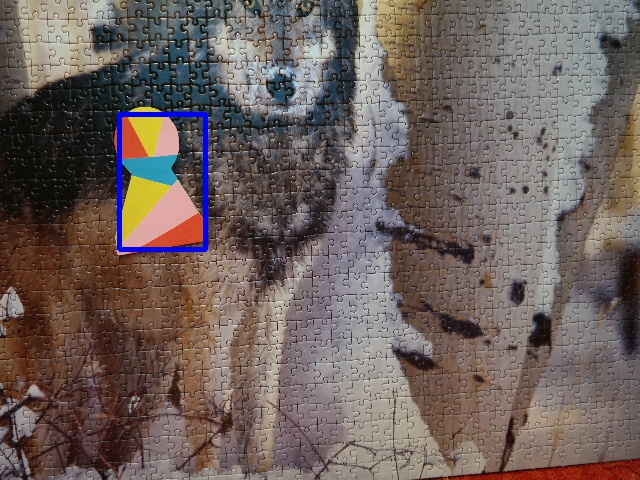
\includegraphics[width=\linewidth]{img/pattern_matching/initial.jpg}
    \caption{Initial image with selected object}
  \end{subfigure}
  \begin{subfigure}{0.48\linewidth}
    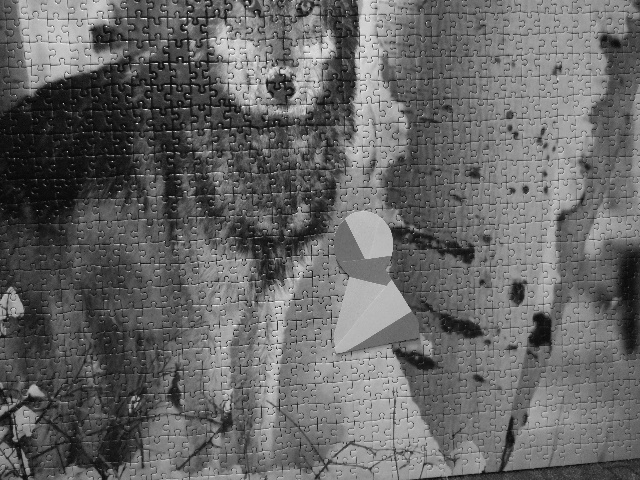
\includegraphics[width=\linewidth]{img/pattern_matching/blackwhite.jpg}
    \caption{Converting it to black white}
  \end{subfigure}
  \begin{subfigure}{0.48\linewidth}
    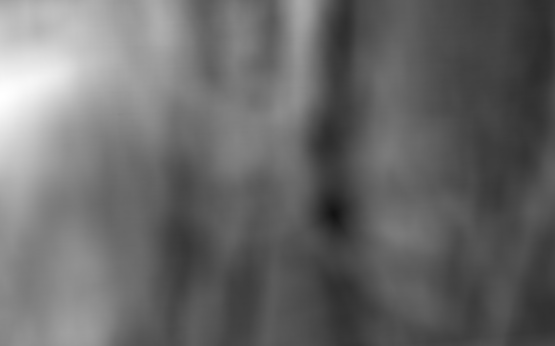
\includegraphics[width=\linewidth]{img/pattern_matching/mask.jpg}
    \caption{Mask created by applying metric}
  \end{subfigure}
  \begin{subfigure}{0.48\linewidth}
    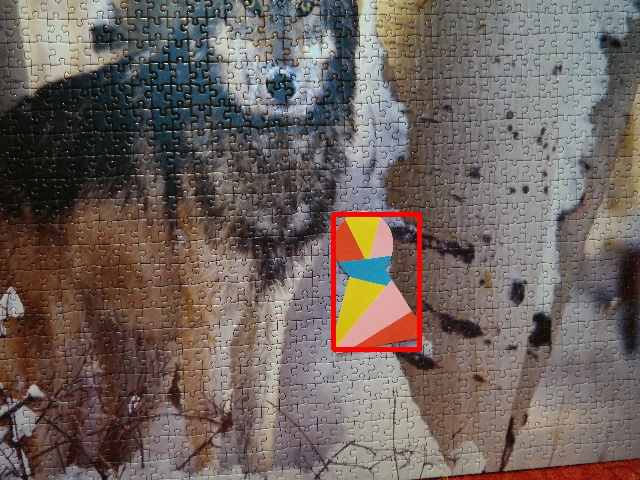
\includegraphics[width=\linewidth]{img/pattern_matching/result-correct.jpg}
    \caption{Darkest point (lowest value) from mask is choosed}
  \end{subfigure}
  \begin{subfigure}{0.48\linewidth}
    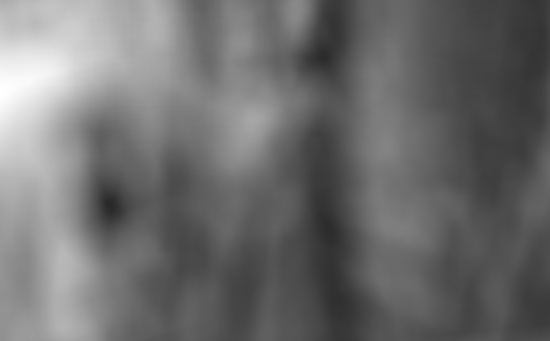
\includegraphics[width=\linewidth]{img/pattern_matching/mask-incorrect.jpg}
    \caption{Mask with darkest point on the left}
  \end{subfigure}
  \begin{subfigure}{0.48\linewidth}
    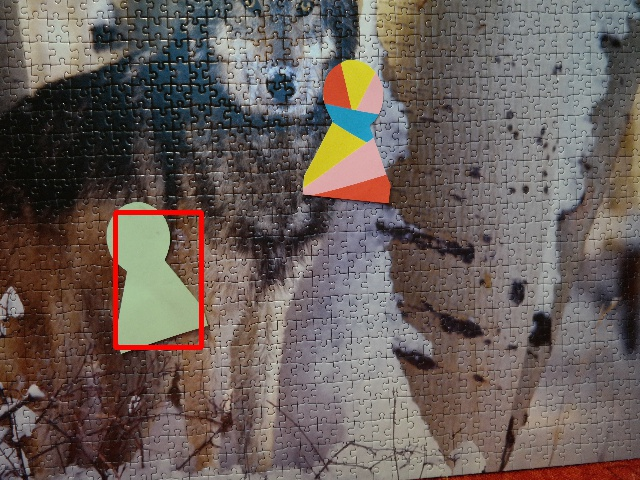
\includegraphics[width=\linewidth]{img/pattern_matching/result-incorrect.jpg}
    \caption{Incorrectly matched pattern}
  \end{subfigure}
  \caption{Process of the pattern matching}
  \label{fig:pattern-matching-tracker}
\end{figure}

%%%%%%%%%%%%%%%%%%%%%%%%%%%%%%%%%%%%%%%%%%%%%

\section{Sequence-based algorithms}

We denote as sequence-based algorithms a class of tracking algorithms, which
are using information from a sequence of images.

Using the advantage of information from previous frames one could create not only
more stable but also faster trackers. Furthermore, trackers of this class usually preserve identity, which means
that also in the case of multiple moving objects in a frame it remains tracking the original
one.

Examples of the information we can obtain from sequence of the images are:
\begin{itemize}
\item velocity -- from previous images we can estimate the speed and direction of
  the movement. This information can reduce the searching area to smaller one
  and increase the speed of the algorithm.
\item appearance -- the object may rotate and change its shape or color. Tracker able to
  learn can be persistable against such changes
\end{itemize}

An algorithm using this information can cope with occlusion (one object covers
another) -- what detection algorithms are usually not able to do.

In the next sections, we will present a few trackers implemented in the OpenCV. We
provide a short overview of the trackers available.

\subsection*{BOOSTING tracker}
\todo[inline]{Citace?}
Boosting tracker is based on online AdaBoost. It considers a bounding box as
a positive sample and patches of background as negative ones. For a new image, the
classifier runs on every pixel in the neighborhood of the previous location,
scoring every pixel. The location with the highest score is chosen as a new
location. The implementation in OpenCV is based on \citet*{boosting}.

\subsection*{MIL tracker}
The MIL is an abbreviation for Multiple Instance Learning. In comparison to the
BOOSTING tracker, it does not keep only one image of the positive example, but a
set of images. The tracker considers a small neighborhood of the
current position as possible positive examples. It helps the tracker to cope with
the occlusion. OpenCV implementation is based on \citet*{mil}.

\subsection*{KCF tracker}
KCF stands for Kernelized Correlation Filters. Similarly, as the MIL tracker,
it uses more positive samples and their large overlapping regions.
Implementation provided by OpenCV is based on \citet*{kcf}.

\subsection*{TLD tracker}
Tracking, learning and detection, these are the three components of the TLD
tracker. The tracker works frame to frame, and detection is run to correct the
tracker if necessary. The learning estimates detector's errors and updates it
to avoid these errors in the future. The implementation in OpenCV is based on
\citet*{tld}.

\subsection*{MEDIANFLOW tracker}
This tracker focuses on forward-backward error trying to minimize it. The
implementation in OpenCV is based on \citet*{medianflow}.

\subsection*{MOSSE tracker}
MOSSE tracker is proposed for fast object tracking using correlation filter
methods. Firstly it does Fast Fourier Transform for template and the image.
Then an convolution operation is performed between the images and the result is
inverted by Inverse Fast Fourier Transform (IFFT). The position is estimated by
the highest value of the IFFT response. More about the tracker is available in
the paper by \citet*{mosse}.

\subsection*{OpenCV note}
OpenCV-contribute implements all above-described sequence-based trackers. An
overview of OpenCV trackers is provided by \citet*{opencv-trackers}.

\subsection*{Correlation tracker}
We decided to include a tracker implemented in Dlib. This
correlation tracker is based on the paper by \citet*{correlation}.

%%%%%%%%%%%%%%%%%%%%%%%%%%%%%%%%%%%%%%%%%%%

\section{Trackers evaluation}

In the previous section, we described many different trackers. Now we provide
their evaluation. The goal is to find the best-performing trackers. The
trackers differ in the approach to obtain information from the video stream, so
it is important to test them under real conditions.

Firstly, we define the key abilities which are essential for our project. Then
we provide a description and the results from several experiments. The
experiments work with only one camera, since in this section we are not
evaluating the localization, but only trackers. At the end of this section, we
provide a few pieces of advice how to choose the best tracker for a specific
environment.

\subsection*{Key abilities of the tracker}

The trackers differ, therefore they can outperform others in some specific
situations. To be able to compare two trackers, we provide a list of the most
important properties in the project.

\begin{itemize}
	\item Accuracy
	\item Speed
	\item Ability to recover from the occlusion
	\item Ability to track multiple objects
\end{itemize}

The following paragraphs describe their importance and also the way we measure them
in our experiments.

\subsubsection*{Accuracy}

A good tracker has to be accurate. The tracker, which is not accurate, does not
satisfy its purpose. Furthermore, the accuracy is important to obtain good
localization results, since the inaccuracy of the estimated position of the
object in the image cause inaccuracy in the estimated position in the 3D space.

It is quite difficult to say what is accuracy in the tracker case. Hence, we
measure \emph{inaccuracy} instead. Inaccuracy in our case is represented by the
distance (in pixels) from the true position of the object and the one provided
by the tracker. Higher values mean less accurate tracker.

To obtain robust results (not depending on one image), we take many images and
compute the inaccuracy for each of them. Then the mean of this inaccuracy is
the estimated inaccuracy for the tracker. The value is dependend on the
resolution of the images. In our case we use images 640 $\times$ 480 px.

The last problem remaining is to get the right position of the object. One
approach is to get the position by selecting the object by a human. This
approach is very time consuming because only a one-minute long video contains
approximately 1800 frames.

Instead of this approach, we select the best tracker. We do it by looking at
the tracking performance on the video of all trackers. Then we choose a one
tracker, which we think perfermed the best (most accurate). This representative
tracker has imprecision equal to 0.  The inaccuracy of the other trackers is
computed as a distance between the selected object by this tracker and the
representative tracker. 

\todo[inline]{Zistit rozptyl vysledkov u accuracy}

\subsubsection*{Speed/Computational time}

Trackers differ not only in their accuracy but naturally also in the time
needed to process an image to find the object. To measure the tracker's speed,
we measure this time. We measure it as a number of ticks passed during calling
tracker update (get the position on the given image). Then we take the number
of the ticks per second and divide it by the number of ticks needed for tracker
update. This way we obtain the number of the images that could be processed in
one second by this tracker. Again, we do it on many images and then take a mean
of these values.

For the number of images that could be processed in one second, we use a
shortcut FPS, coming from Frames Per Second. A higher number means a higher
speed of the tracker, therefore less time needed for each image.

This value is highly dependent on the computer and the operating system.
Therefore, we use the value of FPS as a rough guess.

The results were computed on the a system with Intel(R) Core(TM) i5-7300HQ CPU
(2.50GHz, 2496 Mhz, 4Core), 16GB RAM running Microsoft Windows 10 Enterprise.

Choosing a tracker by its speed is important. We consider a tracker too slow if
it is not able to track live ($>$30~FPS). Even if the tracker has 30~FPS in the
experiment, it might be too slow in the application, since the application has
to perform many other tasks. Slow tracker may use too much computational power,
therefore the application may not run smoothly.

\subsubsection*{Recovering from the occlusion}

We refer to occlusion as a partially or fully coverage of the tracked object by
another object, or leaving the view of the camera.

During the tracking, it might come handy to have a tracker, which can recover
from the occlusion. It is not easy, to keep the object visible in both cameras.
Therefore, we are interested also in the ability to recover from the occlusion.

To test this ability, we watched the videos with tracking results and decided
if the tracker can recover or not.

Another useful ability is to detect if the object is lost. It is better to
report object loss than providing incorrect results. We tested it together with
recovering.

\subsubsection*{Tracking multiple objects}

As an addition to our project, our program can localize multiple objects. When
working with multiple objects, it is important to remember that not all
trackers may be able to track correctly multiple objects at the same time.

Not many trackers can handle if the tracking objects occlude each other.

To decide, if the tracker is able or not to track multiple objects, we watched
tracker's performance and made a decision based on video..

With tracking multiple objects, the speed of the program may decrease rapidly.
It is important to remember, that each object in each camera view has own
tracker. Therefore the tracking part takes more time.

In the next section, we provide an overview of the experiment used to estimate
tracker abilities.

%%%%%%%%%%%%

\subsection{Experiments and the results}

We know describe the experiments useid to measure tracker's statistics. Since the
main use of our project can be to track robots and to record their trajectory,
we decided to test the trackers under similar circumstances.

In some experiments we use an autonomous robot, which has the shape of oval, 3~cm
height and having 6~cm in diameter. This robot is able to follow a black line.
We used an oval as the shape of the line (see the figure \ref{fig:robot-oval}).

In order to test the trackers under same conditions, we recorded a video of the
robot. We then found the bounding box for the object at the start and
initialized the trackers on the same video with same bounding box at the
beginning. We made only some exception because of the requirements of the some
trackers, which are mentioned in the corresponding experiment.

\subsubsection{Speed and accuracy}

The goal of the first experiment is to estimate tracker's speed and accuracy. We used a
video of the robot moving along the oval. For the accuracy measurement we
choosed a Simple Background tracker as our representative, since it provided an
excellent example of the correct tracking on this video. The representative
tracker is always displayed as a red bounding box and the blue is used for the
tested tracker.

Since the Simple Background trackers need an empty background, when
initializing, we passed an image without a robot to it.

\begin{figure}
\centering
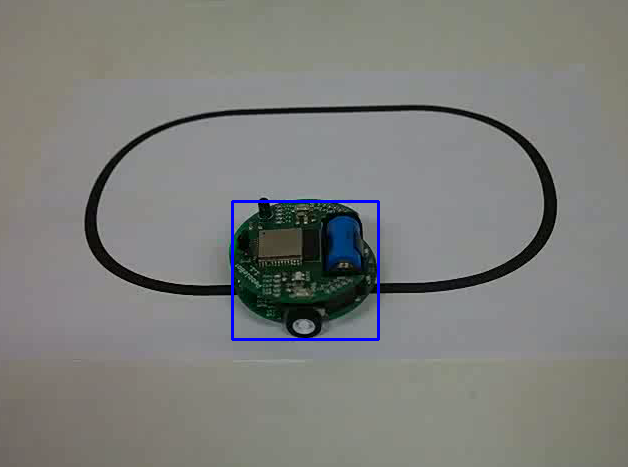
\includegraphics[width=0.6\linewidth]{img/robot-oval.png}
\caption{Selecting object to track on the video}
\label{fig:robot-oval}
\end{figure}

We consider this experiment as quite difficult for the trackers, since the
robot is not only moving, but also quite fast changing its appearance. In a
second or two, its top platform is mirrored. On the other hand, the object does
not change size and the background is very clear.

The results of the experiment are available in the table
\ref{table:experiment-robot}. We provide expected value and standard deviaton
for the inaccuracy, computed for the sample. Both values are in the pixels. For
the HSV tracker we choosed to track the blue battery, which have one-color area.

\begin{table}
\centering
\begin{tabular}{l|l|l|l}
Tracker	& FPS & E(Inaccuracy) & std(Inaccuracy) \\
\hline
\input{experiments/trackers.txt}
\end{tabular}
\caption{Estimation of the trackers speed and inaccuracy.}
\label{table:experiment-robot}
\end{table}

\begin{figure}
\centering
\begin{subfigure}{0.48\linewidth}
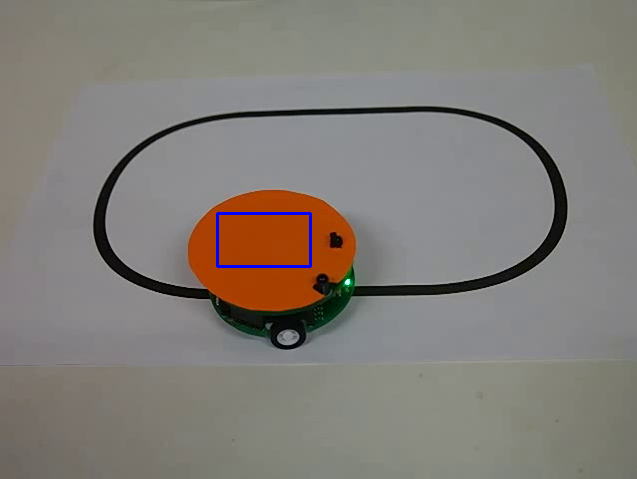
\includegraphics[width=\linewidth]{img/experiments/hsv-select.png}
\caption{Selecting bounding box for HSV tracker}
\label{fig:hsv-bbox}
\end{subfigure}
\begin{subfigure}{0.48\linewidth}
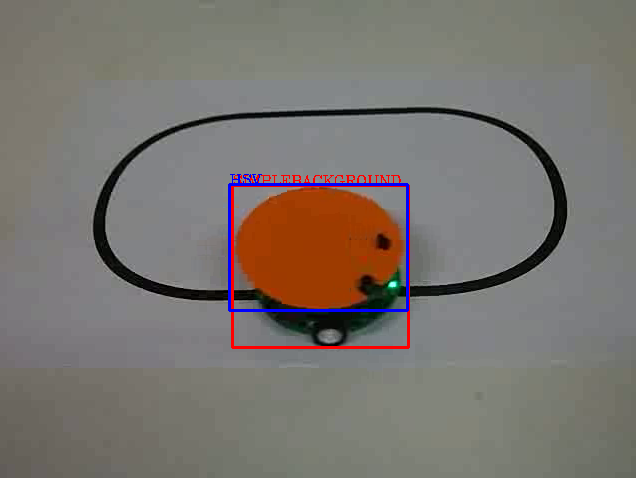
\includegraphics[width=\linewidth]{img/experiments/hsv-tracking.png}
\caption{Simple background tracker (red) and HSV tracker (blue)}
\label{fig:hsv-diff}
\end{subfigure}
\caption{Testing HSV tracker}
\end{figure}

\begin{table}
\centering
\begin{tabular}{l|l|l|l}
Tracker	& FPS & E(Inaccuracy) & std(Inaccuracy) \\
\hline
\input{experiments/hsv.txt}
\end{tabular}
\caption{Estimation of the trackers spped and inaccuracy in the experiment with orange cap.}
\label{table:hsv}
\end{table}

From the results, we can see that MIL, BOOSTING and TLD trackers are too slow
for our application which runs live. HSV tracker is not able to perform at
all, since the robot is multicolored object.

We can also see that, even the MIL and BOOSTING trackers were slow, they
performed quite well. The trackers which have mean value of accuracy more than
100 lost the object at some point and were not aware of it.

As a result from this experiment, we consider CORRELATION, SIMPLEBACKGROUND,
MEDIANFLOW, PATTERMATCHING as usable for our purposes.

To test HSV tracker, we modified the experiment by with placing orange paper to
track on the top of the robot (see figure \ref{fig:hsv-bbox}). The obtained
values for this tracker and the others are listed in the table \ref{table:hsv}.
For improving the performance of the HSV tracker, it is better to select
smaller area with the same color. Therefore, the tracker will track only this
are, not the whole object. The difference between tracked are by Simple
Background tracker and the HSV tracker is displayed in the figure
\ref{fig:hsv-diff}. The red line symbolises Simple Background tracker and the
blue one the HSV tracker.

\todo[inline]{Netusim, ci pisat nazvy trackerov velkym alebo malym, niektore su fakt srkatky, u inych to neviem...}

\subsection{Object under occlusion}

As we have mentioned earlier, it might come handy, to have a tracker which is
able to recover from occlusion. We prepared an experiment, which loose the
robot from the view. We were interested if the tracker is able to report object
lost (or returns wrong results) and if it was able to track the object again
after coming back to camera view. The example of the successful recover from
the occlusion is displayed in the figure \ref{fig:occlusion}.

\todo[inline]{meratelne vysledky?}

\begin{figure}
\centering
\begin{subfigure}{0.48\linewidth}
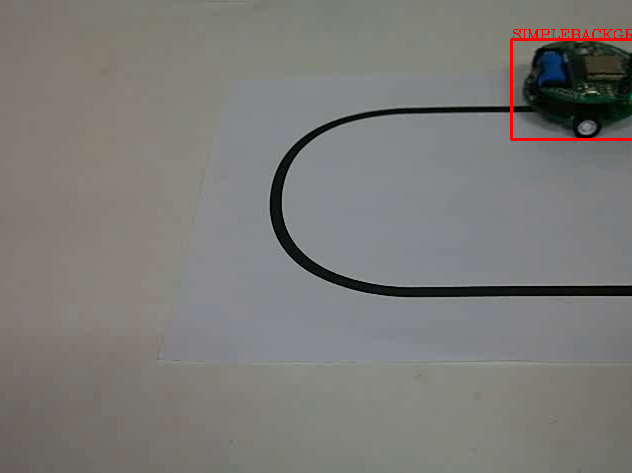
\includegraphics[width=\linewidth]{img/experiments/occlusion1.png}
\end{subfigure}
\begin{subfigure}{0.48\linewidth}
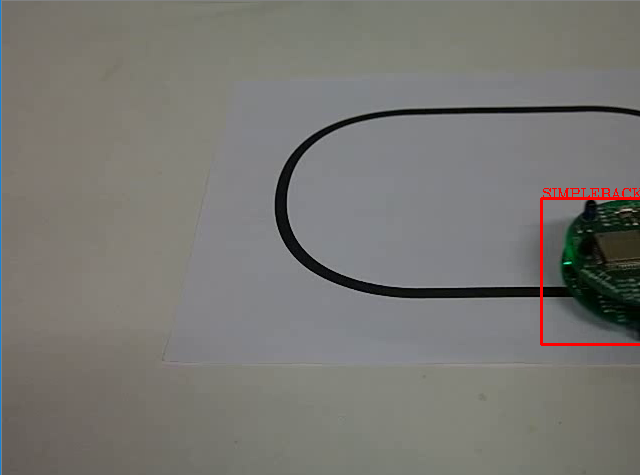
\includegraphics[width=\linewidth]{img/experiments/occlusion2.png}
\end{subfigure}
\caption{Example of successfully recovering from the full occlusion}
\label{fig:occlusion}
\end{figure}

\subsection{Tracking multiple objects}

The last test for the trackers is ability to track multiple objects. Simple
detection-based trackers usually choose the best position with biggest area
satisfing given condition, therefore tracking multiple object may not be possible.

In a situation, when tracking multiple objects is needed, sequence-based
trackers may outperform detection-based trackers. We decided to test their
ability to keep tracking the same object, the results are listed in the table
\ref{table:occlusion-multiple} in the fourth and fifth columns.


\todo[inline]{Tu to chce prepisat}
Most of the trackers are not able to recover from mutual occlusion. Denote as
the first object the object behind and the second the one in front of the
first. Then the second object approach first, the tracker of the first object
learn fase of the changing shape of the object and therefore the tracker start
to track the second object. This situation could not resolve most of the
trackers correctly.

\begin{figure}
\centering
\begin{subfigure}{0.48\linewidth}
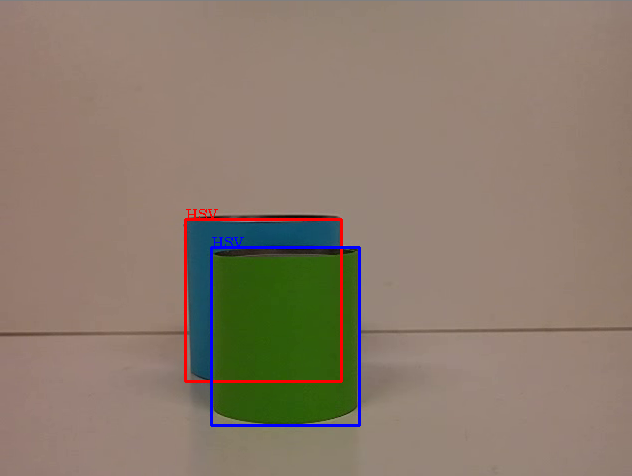
\includegraphics[width=\linewidth]{img/experiments/color-occlusion.png}
\caption{Successful (HSV)}
\end{subfigure}
\begin{subfigure}{0.48\linewidth}
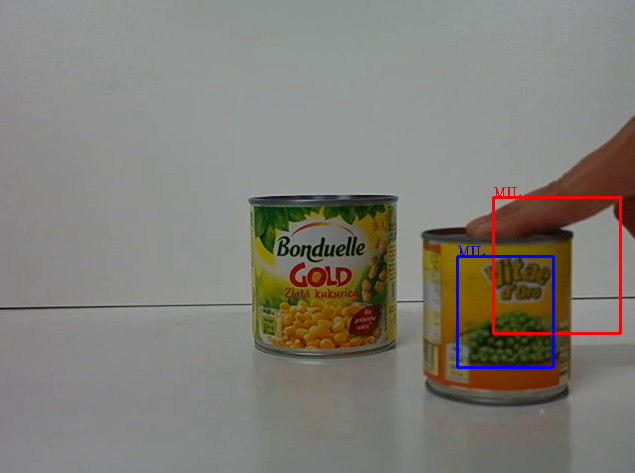
\includegraphics[width=\linewidth]{img/experiments/occlusion.png}
\caption{Unsuccessful (MIL)}
\end{subfigure}
\caption{Example of recoverings from the full occlusion}
\label{fig:occlusion}
\end{figure}

\subsection{Summary}

\todo[inline]{Prepisat}

In the previous section we provided a comparison of the trackers. The goal was
to find the best performing trackers, but the results show, that it might be
better to choose the tracker depending on the environment.

In the speed results we saw, that the trackers MIL, Boosting, TLD were too slow
(less than 30~FPS). Because of their speed, we prefer to not using them.

If the object has an area, which is one-colored, the HSV tracker is a great choice.
The HSV tracker performed very well, it is a fast and stable tracker.
Unfortunately, the disadvantage of this tracker is not only a requirement for
object to have one-colored area, but also this color should not be present in
the background.

If the objects is moving autonomously and the only moving object in the view of
the cameras is the tracked object, then we can use SimpleBackground tracker.

Pattern Matching tracker works well with an objects which preserve the shape
and the size during the tracking.

In conclusion, it is best to try several trackers and find the one, which
perform the best in given envinonmnet. We provide some tips how to find the
best tracker:
\begin{itemize}
\item if the object the only moving object -- use Simple Background
\item if the object has onecolor area -- use HSV
\item if the mutual occlusion of the objects may appear -- try TLD
\item otherwise, it is worth to try MedianFlow, Correlation and sometimes also Mosse and Pattern Matching
\end{itemize}

\begin{landscape}
\begin{table}
\centering
\begin{tabular}{p{5cm}|p{3cm}|p{4cm}|p{5cm}|p{5cm}}
Tracker & Report object lost & Recovers from full occlusion & Ability to track multiple objects & Able to track correctly after mutual occlusion of tracked objects \\
\hline
SIMPLEBACKGROUND & Yes & Yes & No & No \\
MIL & No & No  & Yes & No \\
BOOSTING & No & No & Yes & No \\
TLD & Sometimes & Yes & Yes* & No \\
MEDIANFLOW & Yes & No & Yes & No \\
HSV & Yes & Yes & Only different colors & Yes \\
PATTERNMATCHING & No & Yes & Only different patterns* & Yes \\
CORRELATION & No & No & Yes & No \\
MOSSE & Sometimes & No & Yes & No
\end{tabular}
\vspace{1ex}
\raggedright *Tracker performed badly
\caption{Summary of the trackers abilities}
\label{table:occlusion-multiple}
\end{table}
\end{landscape}

\todo[inline]{Ako sa doslo k Yes/No, dat nejake "cetnosti"}
\todo[inline]{Postavit tunel a urobit experiment s nim}
\todo[inline]{Viacero sa pohybujucich sa objektov s jednym trackovanym}
